% VLDB-Template enhances the ACM master template, acmart.cls v2.19 (2026/06/27):
% https://www.acm.org/publications/proceedings-template
% The ACM Latex guide provides further information about the ACM template
%
% This bundle pins acmart.cls v2.19 (rather than relying on whatever version
% ships with an author's local TeX install or Overleaf project) to guarantee
% consistent formatting across all PVLDB submissions.

\PassOptionsToPackage{table}{xcolor}
\documentclass[sigconf, nonacm, balance=false]{acmart}

%%% do not modify the following VLDB block %%
%%% VLDB block start %%%
\usepackage{pvldb}% VLDB/PVLDB formatting overrides, see pvldb.sty for details.
                      % Do not remove -- required for consistent proceedings
                      % formatting across all VLDB submissions.
%%% VLDB block end %%%

\usepackage{booktabs}
\usepackage{array}
\usepackage{amsmath}
\usepackage{amsthm}
\usepackage{xcolor}
\usepackage{colortbl}
\definecolor{okgreen}{RGB}{226,242,226}
\definecolor{badred}{RGB}{250,222,222}
\usepackage{tikz}
\usetikzlibrary{arrows.meta,positioning,fit,calc,patterns}

\newtheorem{theorem}{Theorem}
\newtheorem{lemma}{Lemma}
\newtheorem{proposition}{Proposition}
\newtheorem{corollary}{Corollary}
\theoremstyle{remark}
\newtheorem{remark}{Remark}
\makeatletter
\setlength\parskip{\z@ \@plus 1.6\p@}
\def\@textbottom{\vskip \z@ \@plus 22\p@}\let\@texttop\relax
\def\thm@space@setup{\thm@preskip=6\p@ \thm@postskip=6\p@}
\usepackage{etoolbox}
\usepackage{needspace}
\usepackage{algorithm}
\usepackage{algpseudocode}
\expandafter\patchcmd\csname\string\proof\endcsname{\topsep6\p@\@plus6\p@\relax}{\topsep6\p@\relax}{}{\typeout{proof patch failed}}
\makeatother

%% The following must be set for each paper (values below are placeholders).
%% Everything else (volume/issue/year defaults, the PVLDB Reference Format
%% block, license footer, and Artifact Availability block) is handled by
%% pvldb.sty -- see that file if you need to change shared defaults.
\renewcommand\vldbdoi{XX.XX/XXX.XX}
\renewcommand\vldbpages{XXX-XXX}
\newcommand{\artifacturl}{https://github.com/adilet-kad/care}
\newcommand{\nruns}{31}
% leave empty if no availability url should be set
\renewcommand\vldbavailabilityurl{\artifacturl}

\begin{document}
\setlength{\textfloatsep}{8pt plus 2pt minus 2pt}
\setlength{\dblfloatsep}{6pt plus 2pt minus 2pt}
\setlength{\dbltextfloatsep}{8pt plus 2pt minus 2pt}
\setlength{\intextsep}{6pt plus 2pt minus 2pt}
\setlength{\abovecaptionskip}{5pt}
\setlength{\belowcaptionskip}{0pt}
\renewcommand{\topfraction}{0.92}
\renewcommand{\bottomfraction}{0.75}
\renewcommand{\textfraction}{0.07}
\renewcommand{\floatpagefraction}{0.80}
\renewcommand{\dbltopfraction}{0.92}
\renewcommand{\dblfloatpagefraction}{0.80}

\title{How Many Data Repairs Can Skip Human Review? Governing Automated
Cleaning under an Error Budget}

%%
%% The "author" command and its associated commands are used to define the authors and their affiliations.
\author{Adilet Kadyrov}
\affiliation{%
  \institution{Pusan National University}
  \city{Busan}
  \country{South Korea}
}
\email{adilet.kadyrov@pusan.ac.kr}

\author{Sofi Nafikova}
\affiliation{%
  \institution{Pusan National University}
  \city{Busan}
  \country{South Korea}
}
\email{nafikovasofi@pusan.ac.kr}

\author{Junyoung Son}
\authornote{Corresponding author.}
\affiliation{%
  \institution{Pusan National University}
  \city{Busan}
  \country{South Korea}
}
\email{jysonpaperinfo@gmail.com}

%%
%% The abstract is a short summary of the work to be presented in the
%% article.
\begin{abstract}
An error in a single cell of a table flows into every report, model and decision built
on it. Automatic data cleaners propose corrections, which we call \emph{repairs}, and
the best of them reach a repair $F_1$-score of $0.86$--$0.97$ on standard benchmarks.
The operator of a production table, however, must decide which repairs may be written
without human review, and an average accuracy says neither which repairs will
be wrong nor how many. In this paper we introduce \emph{error-bounded automation}, the
share of a cleaner's repairs that can be written unreviewed while the error rate among
them stays within a budget the operator sets, with probability $1-\delta$. We realise
it in \textsc{Care}, a governance layer that computes this share from a small
human-checked sample, for any cleaner and without modifying it. On six cleaners and
$21$ cleaner--table pairs the budget held in every configuration, including behind a
real error detector, whereas writing everything unreviewed broke a $5\%$ budget on $12$
of the $21$ pairs. Error-bounded automation ranged from $0$ to $100\%$ and did not
track accuracy. The most accurate cleaner in the study is refused on one table because
it rewrites $176$ cells that were already correct, a cost the $F_1$-score never counts,
and no confidence signal we tested could replace the checked sample. Whether a cleaner
may run unattended is therefore a property of the cleaner and the table together, and
\textsc{Care} measures it before the first unreviewed write.
\end{abstract}

\maketitle

%%% do not modify the following VLDB block %%
%%% VLDB block start %%%
\vldbtopmatter
%%% VLDB block end %%%

\section{Introduction}
\label{sec:intro}

\textbf{Background: cleaners and how they are judged.} A database table is a grid of
\emph{cells}, one value for each row and column. Some cells are wrong, a misspelt city
or a zip code that does not match its state, and we call them \emph{errors}.
\emph{Data cleaning} finds errors and \emph{repairs} them by replacing each wrong value
with the correct one, and we call the systems that do this \emph{cleaners}. Some follow
integrity constraints, the rules a table must obey~\cite{rahm-2000-cleaning,
10.1561/1900000045, 10.1109/icde.2013.6544847, 10.1145/2463676.2465327}, and others
are machine-learning correctors such as Baran~\cite{10.14778/3407790.3407801},
probabilistic systems such as HoloClean~\cite{10.14778/3137628.3137631}, or cleaners
built on large language models (LLMs)~\cite{10.14778/3574245.3574258,
10.14778/3685800.3685890, 10.1145/3698811}. Whatever their design, they are evaluated
the same way, by precision, recall and $F_1$-score averaged over the cells they
repair~\cite{10.14778/2994509.2994518, 10.14778/3675034.3675051, abdelaal-2023-rein}.

\begin{figure}[t]
  \centering
  \resizebox{\linewidth}{!}{% fig_problem.tex: the operator's problem on one real run (Baran on tax, draw 2), and
% what each way of handling the cleaner's repairs does with it at a 5% error budget.
% One column wide. Input from care_main.tex.
% Numbers (csvs/baran_var_tax/2, results_baran_var_tax/2): 121,219 repairs, 14,049 wrong
% (11.6%). Column rate: 87,342 repairs (72%), 1,185 wrong (1.4%). The nine other
% columns: 33,877 repairs (28%), 12,864 wrong (38%), which is 92% of all wrong values.
% At alpha = 0.05 CARE writes the rate column.
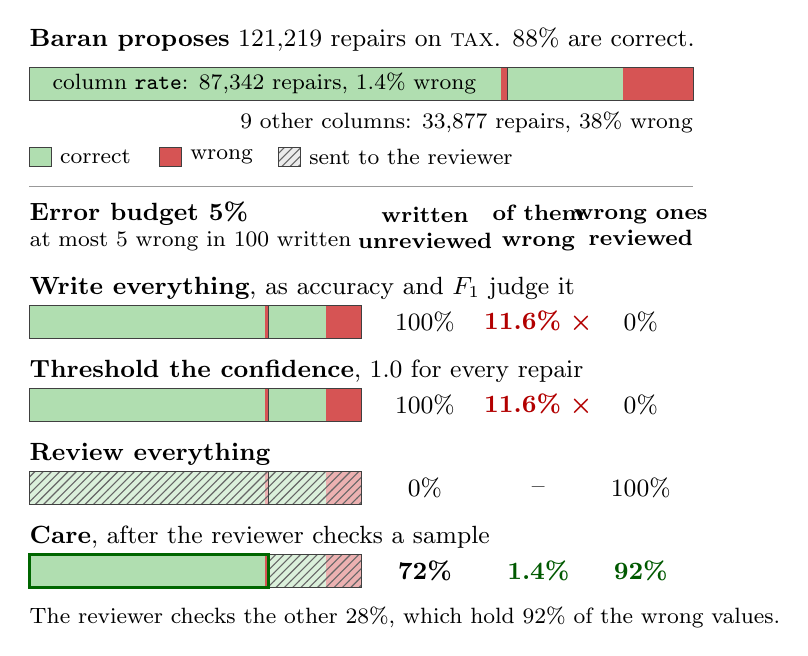
\begin{tikzpicture}[
  font=\small, x=1pt, y=1pt,
  ttl/.style  ={anchor=west, inner sep=0pt, font=\small},
  sml/.style  ={anchor=west, inner sep=0pt, font=\footnotesize},
  num/.style  ={anchor=center, font=\small, inner sep=0pt},
  hdr/.style  ={anchor=center, align=center, font=\footnotesize\bfseries, inner sep=0pt},
]
\definecolor{cgood}{RGB}{176,222,176}
\definecolor{cbad}{RGB}{214,84,84}
\def\H{12}
% \tbar{x}{y}{width}{mode}: the repairs as one bar, correct in green and wrong in red.
% mode 0: all written.  mode 1: all sent to the reviewer.  mode 2: the reliable column
% written, the rest sent to the reviewer.
\newcommand{\tbar}[4]{%
  \pgfmathsetmacro{\wa}{0.7205*#3}\pgfmathsetmacro{\wb}{#3-\wa}%
  \pgfmathsetmacro{\ra}{max(0.0136*\wa,0.9)}\pgfmathsetmacro{\rb}{0.3797*\wb}%
  \fill[cgood] (#1,#2) rectangle ++(\wa-\ra,\H);
  \fill[cbad]  (#1+\wa-\ra,#2) rectangle ++(\ra,\H);
  \fill[cgood] (#1+\wa,#2) rectangle ++(\wb-\rb,\H);
  \fill[cbad]  (#1+#3-\rb,#2) rectangle ++(\rb,\H);
  \ifnum#4=1
    \fill[white, opacity=0.55] (#1,#2) rectangle ++(#3,\H);
    \fill[pattern=north east lines, pattern color=black!60] (#1,#2) rectangle ++(#3,\H);
  \fi
  \ifnum#4=2
    \fill[white, opacity=0.55] (#1+\wa,#2) rectangle ++(\wb,\H);
    \fill[pattern=north east lines, pattern color=black!60] (#1+\wa,#2) rectangle ++(\wb,\H);
  \fi
  \draw[black!75, line width=0.4pt] (#1,#2) rectangle ++(#3,\H);
  \draw[black!75, line width=0.4pt] (#1+\wa,#2) -- ++(0,\H);
}
\def\xa{143}   % share written without review
\def\xe{184}   % error among the written
\def\xr{221}   % share of the wrong values that reach the reviewer

% ---------------- what the cleaner proposes
\node[ttl] at (0,203) {\textbf{Baran proposes} 121{,}219 repairs on \textsc{tax}. 88\% are correct.};
\tbar{0}{181}{240}{0}
\node[sml, anchor=center] at (85,187) {column \texttt{rate}: 87{,}342 repairs, 1.4\% wrong};
\node[sml, anchor=east] at (240,173) {9 other columns: 33{,}877 repairs, 38\% wrong};
% legend
\fill[cgood] (0,157) rectangle ++(8,7); \draw[black!75, line width=0.3pt] (0,157) rectangle ++(8,7);
\node[sml] at (11,160.5) {correct};
\fill[cbad] (47,157) rectangle ++(8,7); \draw[black!75, line width=0.3pt] (47,157) rectangle ++(8,7);
\node[sml] at (58,160.5) {wrong};
\fill[black!8] (90,157) rectangle ++(8,7);
\fill[pattern=north east lines, pattern color=black!60] (90,157) rectangle ++(8,7);
\draw[black!75, line width=0.3pt] (90,157) rectangle ++(8,7);
\node[sml] at (101,160.5) {sent to the reviewer};

\draw[black!40, line width=0.4pt] (0,150) -- (240,150);
\node[ttl] at (0,140) {\textbf{Error budget 5\%}};
\node[sml] at (0,130) {at most 5 wrong in 100 written};
\node[hdr] at (\xa,135) {written\\unreviewed};
\node[hdr] at (\xe,135) {of them\\wrong};
\node[hdr] at (\xr,135) {wrong ones\\reviewed};

% ---------------- lane 1: write everything
\node[ttl] at (0,113) {\textbf{Write everything}, as accuracy and $F_1$ judge it};
\tbar{0}{95}{120}{0}
\node[num] at (\xa,101) {100\%};
\node[num, text=red!70!black] at (\xe,101) {\textbf{11.6\%} $\boldsymbol{\times}$};
\node[num] at (\xr,101) {0\%};

% ---------------- lane 2: confidence threshold
\node[ttl] at (0,83) {\textbf{Threshold the confidence}, 1.0 for every repair};
\tbar{0}{65}{120}{0}
\node[num] at (\xa,71) {100\%};
\node[num, text=red!70!black] at (\xe,71) {\textbf{11.6\%} $\boldsymbol{\times}$};
\node[num] at (\xr,71) {0\%};

% ---------------- lane 3: review everything
\node[ttl] at (0,53) {\textbf{Review everything}};
\tbar{0}{35}{120}{1}
\node[num] at (\xa,41) {0\%};
\node[num] at (\xe,41) {--};
\node[num] at (\xr,41) {100\%};

% ---------------- lane 4: CARE
\node[ttl] at (0,23) {\textbf{\textsc{Care}}, after the reviewer checks a sample};
\tbar{0}{5}{120}{2}
\draw[green!40!black, line width=1.1pt] (0,5) rectangle ++(86.46,\H);
\node[num] at (\xa,11) {\textbf{72\%}};
\node[num, text=green!35!black] at (\xe,11) {\textbf{1.4\%} \checkmark};
\node[num, text=green!35!black] at (\xr,11) {\textbf{92\%}};
\node[sml] at (0,-6) {The reviewer checks the other 28\%, which hold 92\% of the wrong values.};
\end{tikzpicture}
}
  \caption{One run of the cleaner Baran on the \textsc{tax} table at an error budget of
  $5\%$. The top bar shows what the cleaner proposes, coloured by a correctness the
  operator cannot see, and each row shows what one way of handling the repairs writes
  and how many of the wrong values reach the reviewer.}
  \Description{A bar of 121,219 proposed repairs coloured by correctness: one column holds 87,342 repairs of which 1.4 percent are wrong, and nine other columns hold 33,877 repairs of which 38 percent are wrong. Four rows follow. Writing everything and thresholding the confidence both write 100 percent of the repairs with 11.6 percent wrong, over the budget. Reviewing everything puts every wrong value before the reviewer. CARE writes 72 percent with 1.4 percent wrong, within the budget, and the remaining 28 percent, which hold 92 percent of the wrong values, go to the reviewer.}
  \label{fig:problem}
\end{figure}

\textbf{The problem: an average does not tell an operator what to write.} Someone
running a cleaner on a production table must decide, for each proposed repair, whether
to \emph{auto-apply} it, that is, to write it without review, or to \emph{escalate} it
to a human reviewer. An average does not help with that decision, and
Figure~\ref{fig:problem} shows why on one run of Baran on the \textsc{tax} table. Of
its $121{,}219$ repairs $88\%$ are correct, so writing them all puts about $14{,}000$
wrong values into the table, and the average does not say which ones. Reviewing every
repair avoids that at the cost of $121{,}219$ reviews. The average hides a second cost
as well. A cleaner also changes cells that were already correct, and the repair
$F_1$-score, computed only on the known errors, never counts them. The most accurate
cleaner in our study, the LLM-based GIDCL~\cite{10.1145/3698811}, repairs $882$ of
$948$ errors on the \textsc{rayyan} benchmark and at the same time rewrites $176$
correct cells, so that one in five of the values it writes is wrong. No repair metric
reports that figure. A recent study that asked whether automatic repair is ready to
deploy judged it on accuracy~\cite{10.14778/3675034.3675051}. We argue that deployment
is decided repair by repair.

\textbf{The research gap: two existing tools, neither sufficient.} Two existing tools
could answer the operator's question. The first is the \emph{confidence score} that
most cleaners attach to each repair. A threshold on that score bounds the error only if
the score is a probability, and it is not (Section~\ref{sec:conf}). Baran's score, for
one, is the same for every repair (Fig.~\ref{fig:problem}). The second is
\emph{conformal prediction} with \emph{distribution-free risk
control}~\cite{10.1007/b106715, 10.1561/2200000101, 10.1214/24-AOAS1998,
10.1145/3478535}, statistical methods that turn a small checked sample into an error
bound that holds whatever the underlying model. They have been applied to
cleaning~\cite{pmlr-v238-jager24a}, but only to bound \emph{detection}, not the value
that is written, and they assume that the checked sample and the deployed data look
alike, which drift, cleaner updates and poisoned sources all break.

\textbf{Objective and method.} To close this gap we ask a single question. On a given
table, how many of a cleaner's repairs can skip human review at an error rate the
operator chooses? Our answer is \emph{error-bounded automation} $A(\alpha)$, the share
of a cleaner's repairs that can be auto-applied while the error rate among them stays
at most a budget $\alpha$, say $5\%$, with probability at least $1-\delta$, say $90\%$.
To our knowledge the proposed system, \textsc{Care} (Controlled Automation for data
REpair), is the first that computes such a bound for the repairs of an arbitrary,
unmodified cleaner.

\textsc{Care} is a governance layer between the cleaner and the database, and it reads
only the cleaner's output. It changes no repair and makes no cleaner more accurate.
What it adds is a decision, for each repair, between writing it unreviewed and sending
it to the reviewer, taken in three steps. First, it never writes a repair that breaks a
declared integrity rule. Second, it asks the reviewer to check a small random sample
and, from that sample, sets for each \emph{stratum}, a column or a group of columns, the
lowest confidence threshold above which the error can be proven to be below $\alpha$.
Third, it escalates any repair drawn from an untrusted source, whatever its confidence.
On the run of Fig.~\ref{fig:problem} at a $5\%$ budget, these steps write $72\%$ of
the repairs without review, $1.4\%$ of them wrong, and send the other $28\%$ to the
reviewer. Those $28\%$ hold $92\%$ of the cleaner's wrong values, so the reviewer's time
goes to the repairs that need it.

The threshold cannot be set with the usual recipes for risk control, which require an
error that falls steadily as the threshold rises. A cleaner's confidence is neither a
probability nor a reliable ordering, so the error above a threshold does not behave
that way (Sections~\ref{sec:theory} and~\ref{sec:conf}). \textsc{Care} therefore tests
a fixed grid of thresholds with an exact bound~\cite{10.1214/24-AOAS1998}, and it keeps
that bound valid under conditions the test alone does not cover, namely corrupted
sources, overwrites of correct cells and drifting batches.

\textbf{Results.} Because \textsc{Care} never runs a cleaner's code, we governed six
cleaners of four kinds, from a classical corrector to two LLM-based ones, on $21$
cleaner--table pairs. The error budget held in every configuration, including behind a
real error detector and under corruption from untrusted sources, whereas writing
everything unreviewed exceeded a $5\%$ budget in $12$ of the $21$ pairs. The share that
\textsc{Care} admits ranges from nothing to everything for the same cleaner, because
what decides is whether accuracy is \emph{concentrated} in a few large columns, not what
its mean is.

\textbf{Contributions.} In summary, this paper makes three contributions.
\begin{enumerate}
\item \textbf{A deployment criterion and a system that computes it.} We define
error-bounded automation $A(\alpha)$ and build \textsc{Care}, which computes it for any
unmodified cleaner by combining exact rule checking, a per-stratum threshold with a
finite-sample bound, a source-based gate, a label planner and re-validation
(Section~\ref{sec:arch}, Algorithms~\ref{alg:care} and~\ref{alg:plan}).
\item \textbf{A bound that stays valid under corruption.} The bound is retained when
corrupted repairs carry a detectable origin and degrades by at most
$\varepsilon_S(1-\alpha)$ when they do not, even when corruption reaches the checked
sample, and the number of labels a stratum needs is known in advance
(Section~\ref{sec:theory}).
\item \textbf{An evaluation on six cleaners and $21$ cleaner--table pairs, with two
findings that repair metrics miss.} The budget holds in every configuration, and the
admitted share follows how accuracy is distributed over columns
(Section~\ref{sec:results}). Cleaners rewrite correct cells, a cost the $F_1$-score
never counts, and over $\nruns$ runs no confidence signal could replace checked labels
(Section~\ref{sec:findings}).
\end{enumerate}
Section~\ref{sec:related} reviews related work, Section~\ref{sec:setup} defines the
problem, Sections~\ref{sec:arch} and~\ref{sec:theory} present the system and its
bounds, Sections~\ref{sec:exp} to~\ref{sec:findings} report the evaluation, and
Section~\ref{sec:limits} discusses limitations.

\section{Related Work}
\label{sec:related}

\textbf{Data repair systems.} Constraint-, statistics- and knowledge-base-driven repair
\cite{10.14778/3137628.3137631, 10.1145/2463676.2463706, 10.1145/2723372.2749431, 10.1145/2723372.2747646, 10.14778/3476249.3476301, 10.1109/icde.2007.367920}, learning- and corpus-based error detection
\cite{10.1145/3299869.3324956, 10.1145/3299869.3319888, 10.1145/3183713.3196889} and ML-based correction with transfer
\cite{10.14778/3407790.3407801} form the lineage, and we adopt the benchmark suite of
Raha and Baran. Bayesian approaches model attribute dependencies
explicitly~\cite{10597910, pmlr-v130-lew21a}, and BClean+~\cite{11361168} has an LLM
derive BClean's user constraints from each column's semantic type. LLM-based cleaners
prompt a foundation model~\cite{10.14778/3574245.3574258}, retrieve grounding tuples
from a data lake~\cite{10.14778/3685800.3685890}, synthesise cleaning
code~\cite{11107465}, or, in GIDCL~\cite{10.1145/3698811}, have an LLM write per-column
detection and correction functions (repair $F_1$-score $0.86$--$0.97$ on our five
tables). Others learn semantic-domain constraints from table
corpora~\cite{10.1145/3725396} or optimise repairs for the downstream
task~\cite{10.1109/icde65706.2026.00198}. All are evaluated on repair accuracy or
downstream utility, none on the error of the subset applied without review.

\textbf{Per-repair confidence.} Probabilistic repair emits per-cell marginal
probabilities \cite{10.14778/3137628.3137631}, Bayesian repair a
posterior~\cite{10597910}, detection ensembles a classifier
decision~\cite{10.1145/3299869.3324956}, and an LLM's self-assessed confidence is only
partly calibrated~\cite{kadavath2022know, xiong2024llms}. None bounds the error of the
cells written, so \textsc{Care} uses such scores only to order repairs.

\textbf{Selective prediction, deferral and sampled cleaning.} Writing or escalating each
repair is selective classification~\cite{geifman2017selective} and learning to defer to
an expert~\cite{mozannar2020defer}. Those methods train or fit the selector, whereas
\textsc{Care} governs a cleaner it cannot modify, per stratum and under corruption
(Table~\ref{tab:proc} includes their selection rule). SampleClean
\cite{wang2014sampleclean} drew error bounds from a small cleaned sample for aggregate
queries, not for the cells written. Interactive cleaners such as
Falcon~\cite{he2016falcon} and Raha~\cite{10.1145/3299869.3324956} spend a label
budget to \emph{produce} repairs, whereas \textsc{Care}'s labels bound their error.
Data-validation systems~\cite{schelter2018deequ, breck2019tfdv, song2021autovalidate}
check constraints per batch, as \textsc{Care}'s rule check does, and drift detectors~\cite{rabanser2019drift}
flag a changed input distribution, but neither bounds a repair's error. Trust labels on sources follow the provenance
literature~\cite{cheney2009provenance}, and conformal validity under noisy
labels~\cite{einbinder2022noisy} underlies our treatment of label noise.

\textbf{Conformal prediction and risk control.} The closest work applies conformal prediction to tabular cleaning~\cite{pmlr-v238-jager24a}, where a per-column imputation model flags cells outside its prediction set and substitutes its own prediction. This
bounds detection, not the repair written, and assumes \emph{exchangeability}, that is,
that the checked sample and the deployed data follow the same distribution.
Propositions~1--2 treat the case where they do not. A concurrent system~\cite{math14101599}
pairs conformal calibration with rejection of low-confidence corrections under the same
assumption, and conformal bounds for language-model output~\cite{quach2024conformal,
mohri2024conformal} bound the error of generated text, not of database writes.

Our test is fixed-grid Learn-then-Test~\cite{10.1214/24-AOAS1998}, which bounds a
risk on exchangeable data for a model its user controls. \textsc{Care} differs in three
ways. It applies the test to a cleaner it cannot modify and scores every written cell
rather than only the detected errors. It calibrates per
stratum~\cite{vovk2003mondrian, romano2020equalized}, at a label cost that
Section~\ref{sec:zero} measures. Finally, it gates on provenance before calibration, so that
the checked sample stays clean under corruption, a case exchangeability does not
cover~\cite{10.1214/23-AOS2276}. Table~\ref{tab:position} places \textsc{Care} against
these lines of work. Each has one of \textsc{Care}'s properties and none has the
combination, which is what a bound on the writes of an unmodified cleaner requires.

\begin{table*}[t]
  \centering
  \caption{\textsc{Care} against the lines of work it builds on. A dash marks a property
  the line of work does not address.}
  \label{tab:position}
  \small
  \setlength{\tabcolsep}{3.5pt}
  \renewcommand{\arraystretch}{1.0}
  \begin{tabular}{@{}l l l l l l@{}}
  \toprule
  Line of work & Repairs governed & Bound covers & Corrupted sources & Threshold per & Human labels spent on \\
  \midrule
  Repair systems~\cite{10.14778/3137628.3137631, 10.14778/3407790.3407801, 10.1145/3698811}
    & its own & none (accuracy) & -- & -- & training the cleaner \\
  Interactive repair~\cite{10.14778/1952376.1952378, he2016falcon, 10.1145/3299869.3324956}
    & its own & nothing & -- & -- & choosing the repairs \\
  Data validation~\cite{schelter2018deequ, breck2019tfdv, rabanser2019drift}
    & any table & batch rules, not repairs & -- & -- & none \\
  Selective prediction~\cite{geifman2017selective, mozannar2020defer}
    & a model it trains & accepted set (exchangeable) & -- & sometimes & fitting the selector \\
  Conformal cleaning~\cite{pmlr-v238-jager24a, math14101599}
    & its own imputer & detection, not the write & -- & column & calibration \\
  \midrule
  \textbf{\textsc{Care}} & \textbf{any cleaner, unmodified} & \textbf{every cell written}
    & \textbf{yes (Props.~1--2)} & \textbf{stratum} & \textbf{24--105 checked cells} \\
  \bottomrule
  \end{tabular}
\end{table*}

\section{Problem Setup and Threat Model}
\label{sec:setup}

This section states what \textsc{Care} decides and what it promises, first in words,
then in symbols and on an example, and finally under corrupted inputs.

\subsection{What \textsc{Care} decides}
\textbf{In words.} A cleaner proposes repairs. For each one \textsc{Care} decides
whether to write it without review or to send it to the reviewer, and it promises
that, among the repairs it writes, the share of wrong values stays within a budget.

\textbf{The error budget.} The budget $\alpha$ is an input that the operator sets, and
not a score that we report. A budget of $5\%$ means that at most $5$ of every $100$
values written without review may be wrong. Precision, recall and $F_1$-score describe a
cleaner, whereas the budget states what the owner of the table accepts, and
\textsc{Care} is judged on keeping whatever budget is set. We report three budgets,
$5\%$, $10\%$ and $20\%$.

\textbf{Repairs and sources.} A \emph{detector} flags the cells it believes are wrong,
and for each flagged cell $i$ the cleaner emits a \emph{repair}, which consists of a
new value, a \emph{confidence score} $\hat s_i\in[0,1]$ and the \emph{sources} the
value was drawn from. We write $Y_i=1$ if the new value equals the true value and
$Y_i=0$ otherwise, which is unknown until the reviewer checks the repair. Truth here is
the benchmark's clean table. The operator marks each source \emph{trusted} or
\emph{untrusted}, an administrative label such as an allow-list of governed tables. A
repair is \emph{gated} if it names sources and none of them is trusted, and a repair
that names no source is not gated.

\begin{figure*}[t]
  \centering
  \resizebox{0.97\linewidth}{!}{% fig_architecture.tex: the CARE pipeline (input from care_main.tex).
% Needs tikz with arrows.meta, positioning, fit and calc.
\providecommand{\inv}[1]{{\small\color{black!85}#1}}
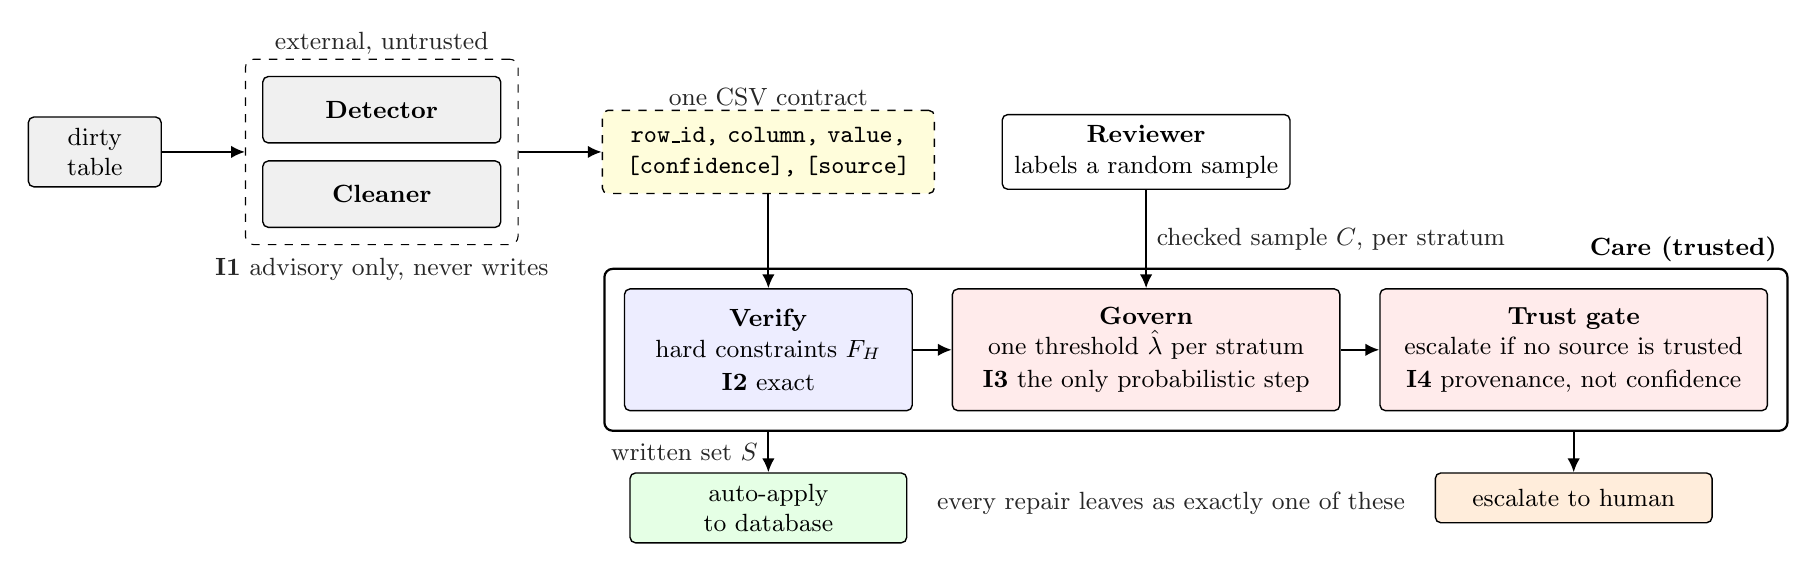
\begin{tikzpicture}[
  font=\small,
  node distance=0pt,
  box/.style    ={draw, line width=0.5pt, rounded corners=2pt, align=center, inner sep=4pt},
  ext/.style    ={box, fill=black!6, text width=78pt, minimum height=24pt},
  stage/.style  ={box, fill=blue!7,  text width=96pt, minimum height=44pt},
  gov/.style    ={box, fill=red!8,   text width=132pt, minimum height=44pt},
  outbox/.style ={box, text width=92pt, minimum height=18pt},
  fl/.style     ={-{Latex[length=5pt,width=4.5pt]}, line width=0.7pt},
  lab/.style    ={font=\small, text=black!85, align=center, inner sep=1.5pt},
  inv/.style    ={font=\small, text=black!85},
]
% ---------- row 1: data, external systems, contract ----------
\node[ext] (det) {\textbf{Detector}};
\node[ext, below=6pt of det] (prop) {\textbf{Cleaner}};
\node[draw, dashed, rounded corners=3pt, inner sep=6pt, fit=(det)(prop)] (extbox) {};
\node[ext, text width=40pt, left=30pt of extbox] (data) {dirty\\table};
\node[lab, anchor=south] at (extbox.north) {external, untrusted};
\node[inv, anchor=north, text width=150pt, align=center] at ([yshift=-1pt]extbox.south)
      {\textbf{I1} advisory only, never writes};
\node[box, dashed, fill=yellow!14, right=30pt of extbox, text width=112pt, minimum height=30pt]
      (contract) {\texttt{row\_id, column, value,}\\\texttt{[confidence], [source]}};
\node[lab, anchor=south] at (contract.north) {one CSV contract};
\draw[fl] (data.east) -- (extbox.west);
\draw[fl] (extbox.east) -- (contract.west);

% ---------- row 2: CARE ----------
\node[stage, below=34pt of contract] (verify)
      {\textbf{Verify}\\hard constraints $F_H$\\[1pt]\inv{\textbf{I2} exact}};
\node[gov, right=14pt of verify] (govern)
      {\textbf{Govern}\\one threshold $\hat\lambda$ per stratum\\[1pt]\inv{\textbf{I3} the only probabilistic step}};
\node[gov, right=14pt of govern] (gate)
      {\textbf{Trust gate}\\escalate if no source is trusted\\[1pt]\inv{\textbf{I4} provenance, not confidence}};
\node[draw, line width=0.8pt, rounded corners=3pt, inner sep=7pt, fit=(verify)(govern)(gate)] (care) {};
\node[font=\small\bfseries, anchor=south east, inner sep=2pt] at ([xshift=-2pt]care.north east) {\textsc{Care} (trusted)};
\draw[fl] (verify.east) -- (govern.west);
\draw[fl] (govern.east) -- (gate.west);
\draw[fl] (contract.south) -- (verify.north);

% ---------- reviewer, above Govern ----------
\node[ext, fill=white, text width=96pt] (human) at (govern |- contract)
      {\textbf{Reviewer}\\labels a random sample};
\draw[fl] (human.south) -- (govern.north)
      node[lab, midway, right=2pt] {checked sample $C$, per stratum};

% ---------- outputs ----------
\node[outbox, fill=green!10, below=22pt of verify.south] (auto) {auto-apply to database};
\node[outbox, fill=orange!14, below=22pt of gate.south]  (esc)  {escalate to human};
\draw[fl] (care.south -| auto) -- (auto.north) node[lab, midway, left=2pt] {written set $S$};
\draw[fl] (care.south -| esc)  -- (esc.north);
\node[lab] at ($(auto.east)!0.5!(esc.west)$)
      {every repair leaves as exactly one of these};
\end{tikzpicture}
}
  \caption{The \textsc{Care} pipeline and the path of one repair from the cleaner to
  the database or to a reviewer.}
  \Description{Block diagram: a dirty table feeds an external detector and cleaner, whose output passes through one CSV contract into CARE (verify, govern, trust gate), which either auto-applies a repair to the database or escalates it to a human.}
  \label{fig:arch}
\end{figure*}

\textbf{Strata and the checked sample.} A \emph{stratifier} assigns each repair to a
\emph{stratum}, in this paper a column, or a group of columns of similar cardinality
when columns are small. Every promise holds per stratum, so a cleaner that is reliable
on one column is trusted on that column only. Within a stratum the repairs split into a
\emph{checked sample} $C$, which the reviewer labels, and a \emph{test set} $T$, on
which \textsc{Care} decides.

\textbf{In symbols.} From the checked repairs that pass the gate,
$C'=\{i\in C:\neg\mathrm{gated}(i)\}$, \textsc{Care} picks one confidence threshold
$\hat\lambda$ per stratum. Three quantities follow.
\begin{align*}
S&=\{i\in T:\hat s_i\ge\hat\lambda\wedge\neg\mathrm{gated}(i)\} &&\text{the repairs written}\\
R(\hat\lambda)&=\Pr(Y=0\mid i\in S) &&\text{the error among them}\\
A(\alpha)&=|S|\,/\,|T| &&\text{error-bounded automation}
\end{align*}
\textsc{Care} chooses $\hat\lambda$ to make $S$ as large as possible subject to
\[
\Pr\bigl[R(\hat\lambda)\le\alpha\bigr]\ge1-\delta ,
\]
where the probability is over the random choice of the checked sample, and it does so
with as few checked labels as possible. A stratum in which some threshold passes is
\emph{admitted}, and its repairs above that threshold are written. When no threshold
passes, \textsc{Care} \emph{refuses} the stratum, $S$ is empty and $A(\alpha)=0$. We
write $R(\alpha)$ for the realised error of the written set, which
Table~\ref{tab:audit} reports beside $A(\alpha)$.

\textbf{A worked example.} A cleaner proposes $100$ repairs on a table with two
columns, $60$ in \texttt{city} and $40$ in \texttt{zip}, each with a confidence score.
The operator sets $\alpha=0.2$ and $\delta=0.1$, and each column is a stratum.
\textsc{Care} draws $24$ repairs from each column for the reviewer to check. In
\texttt{city} all $24$ are correct, just enough to prove an error below $0.2$
(Section~\ref{sec:zero}), so the remaining $36$ \texttt{city} repairs may be written.
In \texttt{zip} $7$ of the $24$ are wrong, no threshold can prove the bound, and the
remaining $16$ \texttt{zip} repairs are escalated. Two \texttt{city} repairs cite an
untrusted source and are escalated whatever their score. \textsc{Care} writes $34$ of
the $52$ repairs it decided, $A(0.2)=0.65$, with the bound that, with probability at
least $0.9$ over the choice of checked sample, the error rate among repairs written this
way is at most $0.2$.

\textbf{Scope.} The bound is on repairs, not detection. It limits the chance that a
value \textsc{Care} \emph{writes} is wrong, and says nothing about the errors the
detector missed or about escalated repairs, which the reviewer decides. It is a statement
about the population of repairs, of which the error measured on a test split is an
estimate.

\subsection{Corruption model}
In deployment, wrong inputs are often systematic rather than random
noise~\cite{10.1145/3774914}. A poisoned source, a broken feed or a cleaner update
each produce repairs that look nothing like the checked sample. We model this as
\emph{contamination}, in which the test repairs split into clean ones $T_c$, drawn the
same way as the checked sample, and corrupted ones $T_a$, which may carry any
confidence and, in the worst case, are all wrong. A corrupted repair is
\emph{detectable} if its sources are marked untrusted, and \emph{undetectable} if it
arrives through a source the operator trusts.

We make two standing assumptions. \textbf{(A1)} The checked sample is labelled
correctly and, per stratum, drawn independently from the same distribution as the
clean test repairs $T_c$. \textbf{(A2)} Corrupted repairs are wrong, $Y_i=0$ for
$i\in T_a$, which is the worst case and makes every bound conservative. A clean repair
wrongly marked untrusted is removed from the checked sample and the test set alike,
which costs automation but never validity. Of the two, (A1) is the assumption that
deployment breaks, because a new source, a cleaner update or a dirtier batch makes the
checked sample stop representing what is decided. Section~\ref{sec:arch} describes
the system that produces $S$ from a cleaner's log under these assumptions, and
Section~\ref{sec:theory} proves what it bounds.

\section{The \textsc{Care} Architecture}
\label{sec:arch}

Section~\ref{sec:setup} fixed what is promised, and this section gives the system
that keeps the promise. Figure~\ref{fig:arch} shows it and Algorithm~\ref{alg:care}
states it line by line. \textsc{Care} sits outside the cleaner, since no cleaner can be
trusted to grade its own repairs. The detector and the cleaner only propose. They never
write to the database, and \textsc{Care} reads their output from a file instead of
running their code. Each proposed repair then passes three steps, and each step makes
one promise.

\textbf{Step 1, \textsc{Verify}} (line~\ref{ln:verify}). \textsc{Care} checks every
repair against the declared \emph{hard constraints}, the rules the table must satisfy.
The check is exact. A repair that breaks a rule is never written, its cell stays
flagged for the reviewer, and the repair is not counted in $A(\alpha)$.

\textbf{Step 2, \textsc{Govern}} (lines~\ref{ln:sample}--\ref{ln:lambda}). In each
stratum the reviewer labels a random sample, and \textsc{Care} sets the lowest
confidence threshold whose error it can prove to be at most $\alpha$. This is the only
step that makes a probabilistic claim, so the proofs of Section~\ref{sec:theory}
concern it alone. The cleaner's confidence serves only to \emph{order} the repairs, and
the checked sample decides where the order is cut. A cleaner that emits the same score
for every repair, as Baran does, is therefore admitted or refused one stratum at a
time.

\textbf{Step 3, the trust gate} (lines~\ref{ln:gatec} and~\ref{ln:gates}). A gated
repair is escalated whatever its confidence. The gate works on the source and not on
the score, and it is applied to the checked sample as well, so that corrupted repairs
cannot shape the threshold.

A repair that passes all three steps is written, and every other repair goes to the
reviewer. Before a batch is committed, a last check re-validates each stratum on a
sample of its own writes (lines~\ref{ln:audit}--\ref{ln:auditend},
Section~\ref{sec:operate}).

\begin{algorithm}[t]
\caption{\textsc{Care} on one batch of proposed repairs}
\label{alg:care}
\small
\begin{algorithmic}[1]
\Require repairs $R$ with scores $\hat s_i$ and sources, budget $\alpha$, failure
  probability $\delta$, grid $\Lambda$, stratifier, trusted sources, hard constraints $F_H$
\Ensure written set $S$ and set $E$ escalated to the reviewer
\State \label{ln:verify}$E\gets\{i\in R: i \text{ violates } F_H\}$,\; $R\gets R\setminus E$ \Comment{Step 1, \textsc{Verify}}
\For{each stratum $g$ of $R$}
  \State \label{ln:sample}draw a checked sample $C_g$ uniformly, the reviewer labels it
  \State \label{ln:gatec}$C'_g\gets\{i\in C_g:\neg\mathrm{gated}(i)\}$ \Comment{Step 3 on the sample}
  \For{$\lambda\in\Lambda$}
    \State $n_\lambda\gets|\{i\in C'_g:\hat s_i\ge\lambda\}|$,\; $k_\lambda\gets$ wrong among them
  \EndFor
  \State \label{ln:lambda}$\hat\lambda_g\gets\min\{\lambda: U(k_\lambda,n_\lambda;\delta/|\Lambda|)\le\alpha\}$, else $+\infty$
        \Comment{Step 2, \textsc{Govern}}
  \State \label{ln:gates}$S_g\gets\{i\in T_g:\hat s_i\ge\hat\lambda_g\wedge\neg\mathrm{gated}(i)\}$
        \Comment{Step 3, trust gate}
  \State \label{ln:audit}audit $n_a$ random repairs of $S_g$, $k$ of them wrong
  \If{$U(k,n_a;\delta)>\alpha$} $S_g\gets\emptyset$ \Comment{re-validation}
  \EndIf\label{ln:auditend}
  \State $S\gets S\cup S_g$,\; $E\gets E\cup(T_g\setminus S_g)$
\EndFor
\end{algorithmic}
{\footnotesize $U(k,n;d)$ is the Clopper--Pearson upper bound at level $d$ for $k$ wrong
out of $n$, and $T_g$ are the repairs of $g$ outside $C_g$. The repairs of $C_g$ and the
audited ones are decided by the reviewer who labels them. The audit needs
$n_a\ge\lceil\ln\delta/\ln(1-\alpha)\rceil$ repairs to pass at all.}
\end{algorithm}

\subsection{Operating \textsc{Care}}
\label{sec:operate}
\textbf{Strata.} Any partition fixed before the checked sample is seen is valid and
changes only how much is written. The default is one stratum per column, and columns
with too few repairs are grouped by cardinality (Section~\ref{sec:strat}).

\textbf{The checked sample.} To be admitted at all, a stratum needs about
$\ln(|\Lambda|/\delta)/\alpha$ checked cells, $24$ at $\alpha=0.2$ and $105$ at $0.05$
(Section~\ref{sec:zero}). The system draws them uniformly per stratum, so the reviewer
does not choose them.

\textbf{Planning the labels.} Before any label is bought, a planner predicts how much
automation a stratum will return for a given number of labels
(Proposition~\ref{thm:floor}) from a $20$-label pilot that is not reused for
calibration, so the strata are fixed before the checked sample is drawn. It escalates outright the
strata that cannot pay for their labels (Algorithm~\ref{alg:plan},
Section~\ref{sec:zero}).

\textbf{Re-validation.} Drift is invisible when the sample is checked. Before a batch
is committed, each stratum is therefore re-validated on a random audit of its own
writes, and it is committed only if the audit alone proves the bound again
(Clopper--Pearson at level $\delta$). Because the audit is a fresh sample of the
writes, the committed stratum's bound then holds at level $\delta$ whatever happened
between calibration and deployment. The rule is conservative on purpose. A stratum
whose error is close to $\alpha$ can fail without any drift, and a failed stratum is
escalated until it is calibrated again, so the audit costs automation and never
correctness (Section~\ref{sec:robust}). An audit must hold at least
$\lceil\ln\delta/\ln(1-\alpha)\rceil$ repairs to pass at all, $45$ at $\alpha=0.05$,
and we use $30$ at the budgets of our drift experiments. Its size does not depend on
the batch, so the operator sets its relative cost through the batch size.
Algorithm~\ref{alg:care} puts the steps together.


\begin{algorithm}[t]
\caption{Planning the labels of one batch}
\label{alg:plan}
\small
\begin{algorithmic}[1]
\Require strata with $m_g$ repairs each, a $20$-label pilot per stratum disjoint
  from every checked sample, $\alpha$,
  $\delta$, review cost $\kappa$ per label
\Ensure for each stratum, a number of labels to buy, a pool to join, or escalation
\For{each stratum $g$}
  \State $p_g\gets$ Beta posterior of the error rate from the pilot
  \State $n_g\gets\arg\max_n\,(m_g-n)\,\mathbb{E}_{p_g}[P_{\mathrm{adm}}(n)]-(\kappa-1)n$
\EndFor
\State calibrate alone every stratum whose expected saving at $n_g$ is positive
\State sort the others with posterior mean below $\alpha$ by that mean
\State pool the prefix of them with the largest positive expected saving
\State escalate every stratum that is neither calibrated nor pooled
\end{algorithmic}
\end{algorithm}

\subsection{Constraint verification}
\label{sec:scalable}

Step 1 must be exact and fast. The rules that matter most in practice are
\emph{functional dependencies} (FDs), where $X\to Y$ says rows that agree on columns
$X$ must agree on $Y$ (a zip code determines its city). Re-evaluating every rule after
each candidate repair takes $18$--$38$\,s per candidate on the $3$M-cell tax table,
depending on the run. \textsc{Care}
instead keeps, per FD, a count of each $Y$ value in every group of rows that agree on
$X$, which a single-cell repair updates in constant
time~\cite{ceri1990deriving}. The index is checked against the reference predicates
when it is built. With it the whole tax queue of about $121{,}000$ repairs verifies in under a
second after a $12$\,s build, at $6$--$14$\,$\mu$s per repair, and build time grows
linearly with the rows.

Which rules to enforce depends on the table's state. On a table that is still dirty, a
correct repair can add a violation because its neighbours are still wrong ($77$ of the
$82$ hospital repairs that add one are correct). The experiments therefore enforce
cell-level completeness and reserve FD enforcement for tables that are already clean,
such as ingestion into a governed warehouse.

\section{Validity of the Bound}
\label{sec:theory}

This section states what the pipeline of Section~\ref{sec:arch} promises. In words, if
the checked sample is drawn the same way as the repairs \textsc{Care} decides, then
with probability at least $1-\delta$ at most a fraction $\alpha$ of the values written
are wrong (Lemma~\ref{lem:ltt}). Propositions~\ref{thm:1} and~\ref{thm:2} extend this
to corruption through untrusted and trusted sources, and Proposition~\ref{thm:floor}
gives the label cost.

\subsection{The base bound, from Learn-then-Test}
\textsc{Care} calibrates with fixed-grid Learn-then-Test (LTT). The candidate
thresholds form a grid $\Lambda$ fixed before any data are seen. Each
$\lambda\in\Lambda$ is tested for ``the error above $\lambda$ exceeds $\alpha$'' with
an exact Clopper--Pearson upper bound~\cite{10.1093/biomet/26.4.404}, that is, the
largest error rate consistent with $k$ wrong out of $n$ checked. The test runs at level
$\delta/|\Lambda|$, the Bonferroni correction that pays for trying $|\Lambda|$
thresholds. Then $\hat\lambda$ is the smallest threshold that passes, or $+\infty$
(escalate all) if none does.

\begin{lemma}[LTT validity \cite{10.1214/24-AOAS1998}]
\label{lem:ltt}
If $C$ and the test cells within a stratum are i.i.d.\ draws from $P$, then
$\Pr[R(\hat\lambda)\le\alpha]\ge 1-\delta$.
\end{lemma}

The grid must be \emph{data-independent}, because thresholds chosen from the observed
calibration values under-cover. The Bonferroni penalty, in contrast, grows only
logarithmically in $|\Lambda|$. With zero observed errors the bound clears $\alpha$
once $n\ge n_{\min}$ (Proposition~\ref{thm:floor}), $105$ labels at $\alpha=0.05$ and
$24$ at $0.2$ (Section~\ref{sec:zero}). Fixed-grid
testing is used rather than risk-controlling prediction sets~\cite{10.1145/3478535} or
conformal risk control~\cite{angelopoulos2024crc} because those need a risk monotone in
$\lambda$, and the selective error of a thresholded cleaner score is not
(Section~\ref{sec:conf}).
In deployment the checked sample is drawn without replacement from a finite batch,
which is more concentrated than i.i.d.\ sampling~\cite{hoeffding1963}, so the bound
remains valid.

\subsection{Detectable corruption}
Suppose first that every corrupted repair comes from a source the operator has marked
untrusted. The gate then removes all of them, and the bound is unchanged.

\begin{proposition}[Retained validity]
\label{thm:1}
Assume (A1)--(A2) and that every $i\in T_a$ is gated, whether or not corrupted repairs
also enter the checked sample. Then the escalation gate removes every corrupted cell
from the auto-applied set, so
$S\subseteq T_c$, $\varepsilon_S:=\Pr(i\in T_a\mid i\in S)=0$, and
$\Pr[R(\hat\lambda)\le\alpha]\ge1-\delta$.
\end{proposition}

\begin{proof}
Every $i\in T_a$ is gated, hence excluded from $S$, so $\varepsilon_S=0$ and
$S=\{i\in T_c':\hat s_i\ge\hat\lambda\}$, with $T_c'$ the clean test repairs that pass
the gate. The gate is a fixed rule on a repair's own fields, so by (A1) $C'$ and $T_c'$
are i.i.d.\ from $P$ conditioned on passing it, and Lemma~\ref{lem:ltt} on $(C',T_c')$
gives the claim.
\end{proof}

The bound depends on whether corruption is detectable and not on its \emph{amount}.

\subsection{Undetectable corruption}
Now suppose that corruption arrives through a trusted source, so the gate cannot see
it. The bound then loosens by the share of corrupted repairs among those written, and by
no more.

\begin{proposition}[Bounded degradation]
\label{thm:2}
Assume (A1)--(A2), and that some corrupted cells carry trusted provenance and may
enter $S$ or the checked sample. Then
$\Pr[\,R(\hat\lambda)\le\alpha+\varepsilon_S(1-\alpha)\,]\ge1-\delta$.
\end{proposition}

\begin{proof}
\predisplaypenalty=0
Condition on membership in $S$ and decompose by cleanliness:
\begin{align*}
R(\hat\lambda)=\;&\underbrace{\Pr(Y{=}0\mid S,\text{clean})}_{=\,R_c(\hat\lambda)}
  \cdot\Pr(\text{clean}\mid S)\\
+\;&\underbrace{\Pr(Y{=}0\mid S,\text{corrupt})}_{=\,1\text{ by (A2)}}
  \cdot\Pr(\text{corrupt}\mid S).
\end{align*}
By definition $\Pr(\text{corrupt}\mid S)=\varepsilon_S$. As in Proposition~\ref{thm:1},
$S\cap T_c$ is the set Lemma~\ref{lem:ltt} controls through $C'$, hence $R_c(\hat\lambda)\le\alpha$ with probability at least $1-\delta$.
Substituting gives $R(\hat\lambda)\le\alpha(1-\varepsilon_S)+\varepsilon_S
=\alpha+\varepsilon_S(1-\alpha)$ on the same event.
\end{proof}

\begin{remark}[Scope and composition]
Proposition~\ref{thm:1} is the case $\varepsilon_S=0$ of
Proposition~\ref{thm:2}. Both hold per stratum, and validity across $m$
strata jointly follows by calibrating each at $\delta/m$.
\end{remark}

\begin{remark}[Corrupted checked sample]
Both proofs use only the \emph{clean} checked repairs. If corrupted repairs also pass
the gate into $C'$, by (A2) each adds a wrong label at every threshold it clears. A
wrong label never lowers a Clopper--Pearson bound, $U(k{+}m,n{+}m)\ge U(k,n)$, so any
threshold admitted on $C'$ is admitted on its clean part, and both propositions hold
as stated.
\end{remark}

The bound on written cells also implies that the table as a whole gets cleaner.

\begin{corollary}[Table-level improvement]
\label{cor:net}
Score every written cell against the truth, an overwritten correct cell counting as an
error. On the event of Lemma~\ref{lem:ltt}, an auto-applied set $S$ of changed cells
removes at least $(1-2\alpha)|S|$ more errors than it introduces, a positive number for
$\alpha<\tfrac12$.
\end{corollary}
\begin{proof}
At most $\alpha|S|$ writes are wrong, and each of them introduces at most one error.
At least $(1-\alpha)|S|$ writes are correct, and each of them removes one error,
because every write is a change.
\end{proof}

\textbf{Label noise.} If the checked labels are themselves wrong at some rate, the
direction of the noise decides~\cite{einbinder2022noisy}. Symmetric noise keeps the
bound at a cost in automation, noise that only turns wrong into correct breaks it, and
calibrating at $\alpha-\bar\eta$ for an upper bound $\bar\eta$ on the noise rate
restores it.


Finally, the bound has a price in labels, which the next result makes exact.

\needspace{9\baselineskip}
\begin{proposition}[Label floor and planner]
\label{thm:floor}
At level $\delta/|\Lambda|$ a stratum is admitted at budget $\alpha$ only if its checked
sample has $n\ge n_{\min}=\lceil\ln(\delta/|\Lambda|)/\ln(1-\alpha)\rceil$ cells,
whatever the cleaner. For a constant score, a stratum of $m$ repairs with error rate
$p$ is admitted from $n$ labels with probability
$P_{\mathrm{adm}}(n)=\Pr[\mathrm{Bin}(n,p)\le k_{\max}(n)]$, with $k_{\max}(n)$ the
largest number of wrong labels whose bound still clears $\alpha$, and buying $n$ labels
at $\kappa$ reviews each saves $(m-n)P_{\mathrm{adm}}(n)-(\kappa-1)n$ reviews in
expectation.
\end{proposition}
\begin{proof}
With no wrong labels the Clopper--Pearson bound is $1-(\delta/|\Lambda|)^{1/n}$, at
most $\alpha$ exactly when $n\ge n_{\min}$, and wrong labels only raise it. With a
constant score every threshold selects the same set, so admission is the single event
that at most $k_{\max}(n)$ labels are wrong, on which the $m-n$ unlabelled repairs are
written unreviewed, while the $n$ labels cost $\kappa n$ reviews against the $n$
reviews they replace.
\end{proof}

\section{Experimental Setup}
\label{sec:exp}

We now describe the tables, the cleaners and the protocol behind every number in
Sections~\ref{sec:results} and~\ref{sec:findings}.

\textbf{Datasets.} We use hospital, beers, flights, rayyan and tax, the standard repair
suite of Raha and Baran~\cite{10.1145/3299869.3324956, 10.14778/3407790.3407801}, drawn
from \cite{10.1109/icde.2013.6544847, 10.14778/2535568.2448943, 10.1186/s13643-016-0384-4,
10.14778/2850578.2850579}. The largest, tax ($200{,}000$ rows, $3$M cells), exercises scale.

\textbf{Cleaners.} Six systems of four kinds, each run in its own environment.
\textsc{Care} never imports their code and reads only a CSV log with the fields
\texttt{row\_id}, \texttt{column}, \texttt{value}, and optionally \texttt{confidence}
and \texttt{source}. \emph{(i)} Baran \cite{10.14778/3407790.3407801}, classical ML.
\emph{(ii)} BClean \cite{10597910}, Bayesian-network inference with user constraints,
and \emph{(iii)} BClean+ \cite{11361168}, the same inference with constraints written
by an LLM. \emph{(iv)} HoloClean \cite{10.14778/3137628.3137631}, factor-graph inference
over denial constraints, the one cleaner whose confidence is a genuine posterior.
\emph{(v)} GIDCL \cite{10.1145/3698811}, in which an LLM writes per-column detection
and correction functions from $20$ labelled tuples. \emph{(vi)}
ZeroEC~\cite{10.1109/ICDE65448.2025.00221}, an LLM cleaner that trains nothing and
works from $10$ user-corrected tuples.

\textbf{How each cleaner was run.} Table~\ref{tab:cover} shows which cleaner--table
pairs are scored, under which detector and confidence signal, and why the rest are not.
Two cleaners could not be run exactly as published. GIDCL's authors release its cleaned
tables but not the code that queried the LLM, so every cell a cleaned table changes is
a proposed repair, and its confidence is the score of its detector, which we retrained
with the authors' code. Our scoring reproduces its paper's $F_1$-score to within
$0.04$, except on \textsc{tax}, where most labelled errors differ from the clean value
only in numeric format. ZeroEC runs from its released code with gpt-4o-mini in place of the larger
models of its paper, and its confidence is the share of three runs that wrote the same
value. It matches its paper on hospital, beers and flights but reaches an $F_1$-score
of $0.11$--$0.30$ on \textsc{rayyan} against $0.81$. Four pairs are $100\%$ accurate on
every error cell they touch. Baran on flights is excluded for that reason and the
others are marked $\dagger$. A register of every deviation accompanies the artifact.


\begin{table}[t]
  \centering
  \caption{How each cleaner was run and which of the five tables are
  scored. \emph{Oracle}: the true error cells are given to the cleaner. Confidence is
  \emph{native} when the cleaner emits it and \emph{ours} when we constructed it.}
  \label{tab:cover}
  \small
  \setlength{\tabcolsep}{3pt}
  \renewcommand{\arraystretch}{0.9}
  \begin{tabular}{@{}>{\raggedright\arraybackslash}p{0.14\linewidth}>{\raggedright\arraybackslash}p{0.28\linewidth}>{\raggedright\arraybackslash}p{0.165\linewidth}>{\raggedright\arraybackslash}p{0.315\linewidth}@{}}
  \toprule
  cleaner & run & confidence & scored / not scored (reason) \\
  \midrule
  Baran & authors' code, oracle detection, $20$ labelled tuples, six unseeded draws & constant $1.0$ (native) & 4 / flights: $100\%$ accurate, excluded \\
  BClean & authors' code and constraint files, oracle & posterior margin (native) & 3 / rayyan, tax: no author constraints \\
  BClean+ & authors' code, flan-t5-xxl constraints, oracle & posterior margin (native) & 3 / rayyan: inference $>100$\,GB; tax: no constraints \\
  HoloClean & authors' code, denial constraints, oracle & posterior (native) & 2 / beers: $711$ of $878$ changes are null imputations outside the gold standard; rayyan, tax: no constraints \\
  GIDCL & released cleaned tables (GPT-4-turbo, Mistral-7B); own detector, retrained by us & detector score (ours); constant on flights & 5 / --- \\
  ZeroEC & released code, gpt-4o-mini for its GPT-4o/3.5 stages, oracle, three runs & run agreement (ours) & 4 / tax: not run \\
  \bottomrule
  \end{tabular}
\end{table}

\textbf{Baselines.} \emph{Apply-all} writes every repair unreviewed. \textsc{Care}
runs with one threshold per stratum (Section~\ref{sec:operate}) and, for comparison in
Section~\ref{sec:strat}, with one threshold for the whole table.

\textbf{Protocol and metrics.} A \emph{split} is one random division of a cleaner's
repairs into a checked sample ($40\%$) and a test set, and a \emph{draw} is one rerun
of Baran, whose sampling is unseeded. $\delta=0.1$ per stratum unless stated otherwise. For each
configuration we report automation $A(\alpha)$ and the \emph{realised error} of the
written set, with a one-sided bootstrap upper bound over $10$--$20$ splits. ``The
budget held'' means that this upper bound is at most $\alpha$. A \emph{refusal}
(``ref.'') is a pair on which nothing is written. Beside every \textsc{Care} number we
report the cleaner's accuracy on error cells. The \emph{human cost} of a batch is
everything the reviewer looks at, that is, the checked sample, the audit and the
escalations together (Table~\ref{tab:labels}).

\textbf{Scoring scope.} Baran, BClean, BClean+, HoloClean and ZeroEC run under
\emph{oracle detection}, in which the true error cells are given, so their
Table~\ref{tab:audit} rows are scored over error cells. GIDCL runs its own detector, so
its rows are scored over every cell it wrote, an overwritten correct cell counting as
an error. Under a real detector (Table~\ref{tab:nonoracle}) every cleaner is scored
that way.


\textbf{Reproducibility.} Every number is read from a result file in the released
artifact (\url{\artifacturl}), which regenerates every table and figure from the cleaner
logs with one command. All sweeps ran on one NVIDIA DGX Spark (GB10, 128\,GB unified memory).

\section{Evaluation: Coverage, Automation and Corruption}
\label{sec:results}

Sections~\ref{sec:results} and~\ref{sec:findings} answer five questions.
\textbf{Q1}~Does the budget hold? Yes, in every configuration, whereas writing
everything unreviewed broke it routinely (Section~\ref{sec:coverage}).
\textbf{Q2}~What decides how much is admitted? How accuracy is distributed across
columns, not its mean, together with the number of checked cells
(Sections~\ref{sec:sep}--\ref{sec:strat}).
\textbf{Q3}~Does the bound survive corruption and drift? Yes through an untrusted
source, and through a trusted one only the contamination is added
(Section~\ref{sec:robust}).
\textbf{Q4}~What does accuracy miss? Cleaners also rewrite correct cells, and this
decides the verdict for the most accurate cleaner (Sections~\ref{sec:harm}
and~\ref{sec:nonoracle}).
\textbf{Q5}~Can a cleaner's confidence replace the checked sample? No
(Section~\ref{sec:conf}).

\subsection{The budget is respected in every configuration}
\label{sec:coverage}
We ran every cleaner on up to five tables, at three budgets, under two stratifications, with
$10$--$20$ splits each. In every one of these configurations the upper bound on the
error of the written set stayed at or below $\alpha$. Written without \textsc{Care},
the same repairs broke the budget in $12$ of the $21$ scored pairs at $\alpha=0.05$
and in $7$ at $\alpha=0.2$ (Table~\ref{tab:audit}, Fig.~\ref{fig:pareto}).

Each row of Table~\ref{tab:audit} reads from left to right. It gives what the cleaner
proposes, the error when all of it is written, and what \textsc{Care} writes at a
budget of $5\%$ and at one of $20\%$. \textsc{Care} does not repair better than the
cleaner. It limits how many wrong repairs are written unreviewed. Writing
nothing would also keep every budget, so the verdict only means something next to the
share written. On average \textsc{Care} wrote $0.35$ of the repairs at
$\alpha=0.05$ and $0.70$ at $\alpha=0.2$. The bound is also conservative in practice.
Of the $1{,}112$ (stratum, split) cells that \textsc{Care} wrote, the realised error
exceeded $\alpha$ in $2$.

\begin{table*}[t]
  \centering  \caption{Every scored cleaner--table pair, without and with \textsc{Care}.
  \textsc{Care} changes no repair. It selects which repairs are written without review.
  $n$ is the number of repairs on true error cells, acc.\ their accuracy, overwr.\ the
  correct cells the cleaner rewrote, \emph{error} the share of wrong values among those
  written, and \emph{written} the share $A(\alpha)$ of repairs written without review.
  Red marks a budget that is broken and green one that is kept. Bold marks where
  \textsc{Care} keeps a budget that writing everything breaks. $\dagger$ is an exactly
  correct cleaner. GIDCL is scored over every cell it wrote, and Baran's rows are medians
  over six draws.}
  \label{tab:audit}
  \normalsize
\setlength{\tabcolsep}{3.2pt}
\renewcommand{\arraystretch}{0.95}
\begin{tabular}{llrrrrrccrrrrc}
\toprule
& & \multicolumn{4}{c}{the cleaner's own repairs} & \multicolumn{3}{c}{\begin{tabular}[b]{@{}c@{}}if every repair\\[-2pt]is written\end{tabular}} & \multicolumn{5}{c}{if only what \textsc{Care} admits is written} \\
\cmidrule(lr){3-6}\cmidrule(lr){7-9}\cmidrule(lr){10-14}
& & & & & & & \multicolumn{2}{c}{budget kept?} & \multicolumn{3}{c}{share written, $A(\alpha)$} & & budget \\
\cmidrule(lr){8-9}\cmidrule(lr){10-12}
Cleaner & Table & $n$ & acc. & $\pi_0$ & overwr. & error & $5\%$ & $20\%$ & $\alpha{=}0.05$ & $0.1$ & $0.2$ & error at $0.2$ & kept? \\
\midrule
Baran & \textsc{hospital} & 500 & 0.909 & 0.683 & 0 & $0.092$ & \cellcolor{badred}$\boldsymbol{\times}$ & \cellcolor{okgreen}\checkmark & $0$ & $0.01$ & $0.58$ & $0.057$ & \cellcolor{okgreen}\checkmark \\
Baran & \textsc{beers} & 3{,}316 & 0.864 & 0.019 & 0 & $0.136$ & \cellcolor{badred}$\boldsymbol{\times}$ & \cellcolor{okgreen}\checkmark & $0.36$ & $0.72$ & $0.80$ & $0.037$ & \cellcolor{okgreen}\checkmark \\
Baran & \textsc{flights}$^{\dagger}$ & 4{,}920 & 1.000 & 1.000 & 0 & \multicolumn{8}{c}{\emph{excluded (nothing to govern)}} \\
Baran & \textsc{rayyan} & 422 & 0.908 & 0.035 & 0 & $0.093$ & \cellcolor{badred}$\boldsymbol{\times}$ & \cellcolor{okgreen}\checkmark & $0$ & $0.27$ & $0.69$ & $0.042$ & \cellcolor{okgreen}\checkmark \\
Baran & \textsc{tax} & 121{,}219 & 0.914 & 0.728 & 0 & $0.086$ & \cellcolor{badred}$\boldsymbol{\times}$ & \cellcolor{okgreen}\checkmark & $0.72$ & $0.73$ & $0.83$ & $0.008$ & \cellcolor{okgreen}\checkmark \\
\addlinespace[1.5pt]
BClean & \textsc{hospital}$^{\dagger}$ & 398 & 1.000 & 1.000 & 0 & $0.000$ & \cellcolor{okgreen}\checkmark & \cellcolor{okgreen}\checkmark & $0.73$ & $0.73$ & $1.00$ & $0.000$ & \cellcolor{okgreen}\checkmark \\
BClean & \textsc{beers} & 2{,}743 & 0.738 & 0.000 & 17 & $\mathbf{0.262}$ & \cellcolor{badred}$\boldsymbol{\times}$ & \cellcolor{badred}$\boldsymbol{\times}$ & $0$ & $0$ & $0.02$ & $\mathbf{0.017}$ & \cellcolor{okgreen}\checkmark \\
BClean & \textsc{flights} & 2{,}522 & 0.500 & 0.000 & 156 & $\mathbf{0.497}$ & \cellcolor{badred}$\boldsymbol{\times}$ & \cellcolor{badred}$\boldsymbol{\times}$ & $0.12$ & $0.12$ & $0.19$ & $\mathbf{0.034}$ & \cellcolor{okgreen}\checkmark \\
\addlinespace[1.5pt]
BClean+ & \textsc{hospital}$^{\dagger}$ & 408 & 1.000 & 1.000 & 0 & $0.000$ & \cellcolor{okgreen}\checkmark & \cellcolor{okgreen}\checkmark & $0.73$ & $0.73$ & $1.00$ & $0.000$ & \cellcolor{okgreen}\checkmark \\
BClean+ & \textsc{beers} & 3{,}327 & 0.781 & 0.034 & 16 & $\mathbf{0.220}$ & \cellcolor{badred}$\boldsymbol{\times}$ & \cellcolor{badred}$\boldsymbol{\times}$ & $0$ & $0.01$ & $0.50$ & $\mathbf{0.123}$ & \cellcolor{okgreen}\checkmark \\
BClean+ & \textsc{flights} & 3{,}919 & 0.783 & 0.000 & 81 & $\mathbf{0.215}$ & \cellcolor{badred}$\boldsymbol{\times}$ & \cellcolor{badred}$\boldsymbol{\times}$ & $0.38$ & $0.50$ & $0.50$ & $\mathbf{0.028}$ & \cellcolor{okgreen}\checkmark \\
\addlinespace[1.5pt]
GIDCL & \textsc{hospital} & 507 & 0.945 & 0.536 & 0 & $0.054$ & \cellcolor{badred}$\boldsymbol{\times}$ & \cellcolor{okgreen}\checkmark & $0$ & $0.17$ & $1.00$ & $0.054$ & \cellcolor{okgreen}\checkmark \\
GIDCL & \textsc{beers} & 3{,}351 & 0.984 & 0.038 & 7 & $0.019$ & \cellcolor{okgreen}\checkmark & \cellcolor{okgreen}\checkmark & $0.72$ & $0.74$ & $1.00$ & $0.018$ & \cellcolor{okgreen}\checkmark \\
GIDCL & \textsc{flights} & 4{,}815 & 0.987 & 0.413 & 29 & $0.020$ & \cellcolor{okgreen}\checkmark & \cellcolor{okgreen}\checkmark & $0.64$ & $1.00$ & $1.00$ & $0.019$ & \cellcolor{okgreen}\checkmark \\
GIDCL & \textsc{rayyan} & 932 & 0.946 & 0.775 & 176 & $\mathbf{0.203}$ & \cellcolor{badred}$\boldsymbol{\times}$ & \cellcolor{badred}$\boldsymbol{\times}$ & \multicolumn{4}{c}{\emph{refused at every $\alpha$}} & \cellcolor{okgreen}\checkmark \\
GIDCL & \textsc{tax} & 2{,}924 & 0.961 & 0.868 & 22 & $0.046$ & \cellcolor{okgreen}\checkmark & \cellcolor{okgreen}\checkmark & $0.33$ & $0.83$ & $0.87$ & $0.008$ & \cellcolor{okgreen}\checkmark \\
\addlinespace[1.5pt]
HoloClean & \textsc{hospital}$^{\dagger}$ & 232 & 1.000 & 1.000 & 0 & $0.000$ & \cellcolor{okgreen}\checkmark & \cellcolor{okgreen}\checkmark & $0$ & $0.72$ & $1.00$ & $0.000$ & \cellcolor{okgreen}\checkmark \\
HoloClean & \textsc{beers}$^{\dagger}$ & 121 & 1.000 & 1.000 & \textemdash & \multicolumn{8}{c}{\emph{excluded (nothing to govern)}} \\
HoloClean & \textsc{flights} & 2{,}337 & 0.742 & 0.000 & 1 & $\mathbf{0.259}$ & \cellcolor{badred}$\boldsymbol{\times}$ & \cellcolor{badred}$\boldsymbol{\times}$ & $0.65$ & $0.68$ & $0.68$ & $\mathbf{0.014}$ & \cellcolor{okgreen}\checkmark \\
\addlinespace[1.5pt]
ZeroEC & \textsc{hospital} & 488 & 0.967 & 0.826 & 0 & $0.030$ & \cellcolor{okgreen}\checkmark & \cellcolor{okgreen}\checkmark & $0$ & $0.92$ & $1.00$ & $0.030$ & \cellcolor{okgreen}\checkmark \\
ZeroEC & \textsc{beers} & 3{,}336 & 0.995 & 0.281 & 0 & $0.005$ & \cellcolor{okgreen}\checkmark & \cellcolor{okgreen}\checkmark & $0.93$ & $0.93$ & $1.00$ & $0.005$ & \cellcolor{okgreen}\checkmark \\
ZeroEC & \textsc{flights} & 4{,}891 & 0.996 & 0.409 & 0 & $0.004$ & \cellcolor{okgreen}\checkmark & \cellcolor{okgreen}\checkmark & $1.00$ & $1.00$ & $1.00$ & $0.003$ & \cellcolor{okgreen}\checkmark \\
ZeroEC & \textsc{rayyan} & 912 & 0.303 & 0.000 & 0 & $\mathbf{0.690}$ & \cellcolor{badred}$\boldsymbol{\times}$ & \cellcolor{badred}$\boldsymbol{\times}$ & \multicolumn{4}{c}{\emph{refused at every $\alpha$}} & \cellcolor{okgreen}\checkmark \\
\midrule
\multicolumn{7}{l}{pairs that break the budget (of $21$)} & $\mathbf{12}$ & $\mathbf{7}$ & & & & & $\mathbf{0}$ \\
\multicolumn{9}{l}{average share written, $A(\alpha)$, over the $21$ pairs} & $\mathbf{0.35}$ & $\mathbf{0.51}$ & $\mathbf{0.70}$ & & \\
\bottomrule
\end{tabular}

\end{table*}

\subsection{Automation depends on where a cleaner is right}
\label{sec:sep}

Does the admitted share follow the cleaner, the table or the accuracy? None of the
three on its own (Table~\ref{tab:audit}, Fig.~\ref{fig:mech}b,c). The same cleaner,
GIDCL, is refused on \textsc{rayyan} and admitted in full on \textsc{beers} and
\textsc{flights} at $\alpha=0.2$. Nineteen of the $21$ pairs admit a non-empty set at
that budget, and the two refusals, both on \textsc{rayyan}, are the right verdict,
since one in five of GIDCL's writes there is wrong (Section~\ref{sec:harm}), as are two
in three of ZeroEC's on the smaller model we could run (Section~\ref{sec:exp}). That
refusal is a verdict on our run, not on ZeroEC as published.

\begin{figure*}[t]
  \centering
  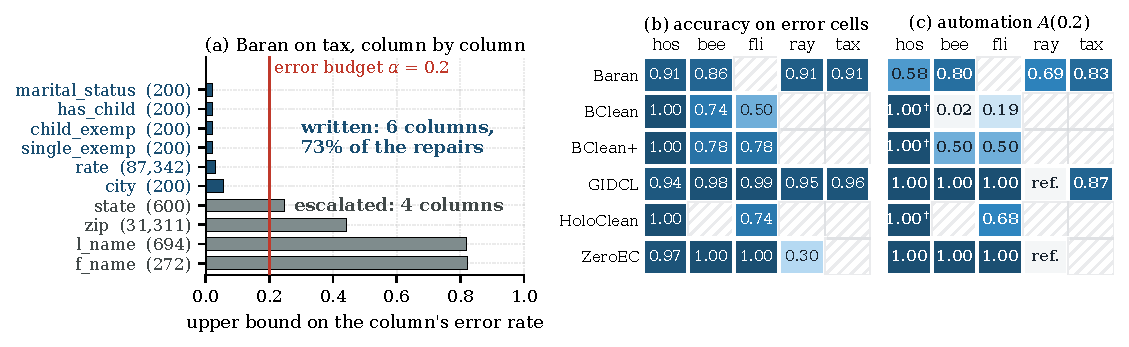
\includegraphics[width=0.96\linewidth]{figures/fig_mechanism}
  \caption{(a) Upper bound on each column's error for Baran on tax (the run of
  Fig.~\ref{fig:problem}), with the
  number of repairs per column; (b) accuracy and (c) error-bounded automation $A(0.2)$ of every
  scored pair (hatched: not scored, ``ref.'': refused).}
  \Description{Three panels: (a) a bar chart of upper bounds on per-column error rates for Baran on tax; (b) and (c) two cleaner-by-table matrices, coloured by accuracy and by error-bounded automation respectively.}
  \label{fig:mech}
\end{figure*}

What decides is how accuracy is \emph{distributed} over columns. Admission is per
stratum, so a cleaner earns automation in the columns where it is reliably right.
BClean on beers is $0.738$ accurate, but no single column is reliable, and
\textsc{Care} writes $0.02$ of its repairs. Baran on tax is the opposite case. Its
accuracy ranges from $0.732$ to $0.956$ over six draws, yet $A(0.1)$ is $0.73$ in five
of them, because the same five columns clear that budget every time while \texttt{zip},
a quarter of the repairs, does not. Fig.~\ref{fig:mech}(a) shows the run of
Fig.~\ref{fig:problem} at $\alpha=0.2$, where a sixth small column is also written. At
that budget two of the six draws admit \texttt{zip} as well, which is why the median
share in Table~\ref{tab:audit} rises to $0.83$.

One number that can be tallied on a small labelled sample summarises this. The
\emph{ceiling} at budget $\alpha$ is the share of a cleaner's repairs in columns whose
error is at most $\alpha$, and $A(\alpha)$ cannot exceed it when strata are admitted
whole. Whether a cleaner may run unattended is therefore a property of the
cleaner--table pair.

\subsection{A stratum needs enough checked cells}
\label{sec:zero}

Being right in a column is not enough. The column must also hold enough checked cells
to prove it. Even with no error observed, a stratum is admitted only from $n_{\min}$
checked cells, $105$ at $\alpha=0.05$ and $24$ at $0.2$
(Proposition~\ref{thm:floor}). HoloClean shows this without confounds. It is correct on
all $232$ repairs it proposes on hospital and still admits nothing at $\alpha=0.05$,
because $93$ checked cells cannot rule out a $5\%$ error rate. At that budget nine
pairs admit nothing, seven because their error is above the budget and two because of
this floor.

\begin{table}[t]
  \centering
  \caption{Alternatives to the default test on the $21$ scored pairs ($10$ splits,
  three budgets, $\delta=0.1$). Mean automation, the splits and (stratum, split) cells
  whose written error exceeded $\alpha$, and the fewest error-free checked cells that
  admit a stratum at $\alpha=0.05$.}
  \label{tab:proc}
  \small
  \setlength{\tabcolsep}{3pt}
  \begin{tabular}{@{}>{\raggedright\arraybackslash}p{0.52\linewidth}rrrr@{}}
  \toprule
  procedure & $\bar A$ & splits & cells & floor \\
  \midrule
  \textbf{default}: $21$ thresholds, Clopper--Pearson at $\delta/21$ & \textbf{0.535} & \textbf{0/630} & 2/1{,}112 & 105 \\
  default at $\delta/m$ over $m$ strata (joint validity) & 0.498 & 0/630 & 2/1{,}034 & 118--132 \\
  declared $|\Lambda|$ ($=1$ for a constant score), one test at $\delta$ & 0.579 & 2/630 & 6/1{,}328 & 45 \\
  SGR selection~\cite{geifman2017selective}, $\lceil\log_2 n\rceil$ bisection tests & 0.509 & 0/630 & 3/1{,}136 & 83 \\
  default with a Hoeffding bound & 0.281 & 0/630 & 0/530 & 1{,}070 \\
  fixed-sequence LTT~\cite{10.1214/24-AOAS1998} from $\lambda=1$ down & 0.282 & 2/630 & 5/788 & 45 \\
  fixed-sequence LTT from $\lambda_0=0.5$ & 0.570 & 4/630 & 11/1{,}371 & 45 \\
  \bottomrule
  \end{tabular}
\end{table}

\textbf{Other tests.} The floor is the price of the test, and Table~\ref{tab:proc}
compares the default with six other valid procedures. A cleaner whose score is
constant by design, such as Baran, or absent, as in GIDCL's log, needs one test instead of $21$, which lowers the
floor to $45$ cells and raises mean automation from $0.535$ to $0.579$. Its largest
effect is on GIDCL on \textsc{rayyan}, which the default refuses at every budget and
the single test admits in part at $\alpha=0.2$ ($0\to0.52$), while both refuse it at
$0.05$ and $0.1$. The other alternatives lose automation or validity. The grid cannot be chosen after
looking at the checked sample without breaking the bound, so the single test is valid
only when the cleaner's design fixes the score in advance. We therefore keep one
default for every reported number, valid for any score, and the rows of
Table~\ref{tab:audit} for Baran and GIDCL are lower bounds. The grid size and $\delta$, the two settings of the default test,
change only how much is written. Over grids of $5$, $17$ and $50$ thresholds and $\delta$ of $0.05$, $0.1$ and
$0.2$, on four pairs at $\alpha=0.2$, the budget held in all $360$ runs, and automation
moved by at most $0.26$, most for BClean+ on beers, whose informative score gains
from a finer grid.

\begin{table}[t]
  \centering
  \caption{Human cost per $100$ repairs with the planner's labels ($\kappa=1$, pilot
  charged) on the ten constant-score pairs. \emph{Labels} are the cells the reviewer checks,
  and \emph{all} adds the escalations.}
  \label{tab:labels}
  \small
  \setlength{\tabcolsep}{4pt}
  \renewcommand{\arraystretch}{0.93}
  \begin{tabular}{@{}ll rr rr rr@{}}
  \toprule
  & & \multicolumn{2}{c}{$\alpha=0.05$} & \multicolumn{2}{c}{$\alpha=0.1$} & \multicolumn{2}{c}{$\alpha=0.2$} \\
  \cmidrule(lr){3-4}\cmidrule(lr){5-6}\cmidrule(l){7-8}
  cleaner & table & labels & all & labels & all & labels & all \\
  \midrule
  Baran & \textsc{hospital} & 63 & 100 & 49 & 94 & 30 & 41 \\
  Baran & \textsc{beers} & 27 & 63 & 16 & 32 & 13 & 26 \\
  Baran & \textsc{flights} & 12 & 12 & 6 & 6 & 3 & 3 \\
  Baran & \textsc{rayyan} & 48 & 100 & 44 & 86 & 40 & 44 \\
  Baran & \textsc{tax} & 1.9 & 29 & 0.8 & 28 & 0.4 & 27 \\
  GIDCL & \textsc{hospital} & 61 & 100 & 43 & 91 & 28 & 34 \\
  GIDCL & \textsc{beers} & 24 & 33 & 14 & 18 & 6 & 6 \\
  GIDCL & \textsc{flights} & 20 & 25 & 8 & 8 & 4 & 4 \\
  GIDCL & \textsc{rayyan} & 44 & 48 & 30 & 39 & 23 & 30 \\
  GIDCL & \textsc{tax} & 20 & 28 & 15 & 23 & 13 & 20 \\
  \bottomrule
  \end{tabular}
\end{table}

\textbf{Planning the labels.} The floor also tells the operator what labels will
return before buying them. On the ten constant-score pairs the planner of
Section~\ref{sec:operate} predicts automation to within $0.034$. With its pilot
charged, it saves $0.60$ of the review queue against $0.41$ for the fixed $40\%$ split
used elsewhere in this section, with half the labels (Table~\ref{tab:labels}).

\textbf{What the labels cost.} A checked cell is a review that would have happened
without \textsc{Care}, so the worst case is the cost of reviewing everything and never
more, and no entry of Table~\ref{tab:labels} exceeds $100$ reviews per $100$ repairs.
The floor depends on the budget and not on the size of the stratum, so the cost falls
with volume. Tax needs about $240$ labels, $0.2\%$ of its queue, whereas hospital, with
${\sim}500$ repairs over $17$ columns, leaves most of its queue to the reviewer at
$\alpha=0.05$. A few thousand repairs are already enough. On flights, where each
cleaner proposes $2{,}337$ to $4{,}891$ repairs, all five scored cleaners are admitted
in part at that budget (Table~\ref{tab:audit}). The planner reports this before any label is bought, and the artifact
lists the stratum sizes below which labelling does not pay.

\subsection{The ceiling predicts automation under controlled corruption}
\label{sec:sweep}

Ni et al.~\cite{10.14778/3675034.3675051} release versions of the benchmark tables
corrupted at controlled rates. We ran Baran on sixteen of them (four tables, cell error
rates $0.07$--$0.49$) and recorded each stratum's ceiling before any calibration. The
budget held in all $336$ configurations, while Baran's accuracy fell from $0.771$ to
$0.055$ and the error of writing everything climbed to $0.94$
(Fig.~\ref{fig:sweep}). Automation did not simply fall with accuracy. On beers it rose
while accuracy fell from $0.42$ to $0.16$. It followed the ceiling instead, equalling
it on $140$ of $168$ draw--budget rows and never exceeding it.

\begin{figure}[t]
  \centering
  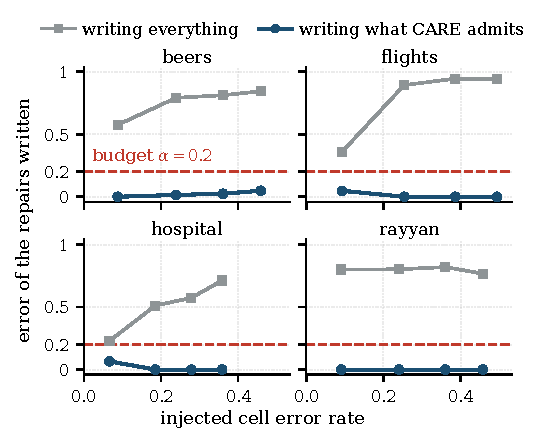
\includegraphics[width=\linewidth]{figures/fig_corruption}
  \caption{Error of the repairs written against the injected error rate, for Baran on
  four tables (Ni et al.'s variants, medians over draws).}
  \Description{Four small line charts, one per table, of the error of written repairs against the injected cell error rate: apply-all rises towards one while CARE stays below the budget line.}
  \label{fig:sweep}
\end{figure}

\subsection{A threshold per column is a trade-off}
\label{sec:strat}
One threshold per stratum is not always better than one for the whole table, which we
call \emph{marginal} control. On tax Baran's score is constant, so marginal control
admits all or nothing. On a draw whose pooled error is $0.268$ it admits nothing, whereas per-stratum
control admits $0.72$--$0.73$ at $\alpha\le0.1$ with an error of at most $0.014$, because it isolates the
five reliable columns from \texttt{zip}. On hospital the trade reverses. At
$\alpha=0.2$ marginal control writes everything at error $0.083$ and per-stratum control
writes only $0.58$, because ${\sim}500$ repairs over $17$ columns leave every stratum
thin. Stratification pays when reliability differs across strata \emph{and} the strata
are large enough to calibrate, and both can be checked in advance from the ceiling and
the stratum sizes.

\begin{figure}[t]
  \centering
  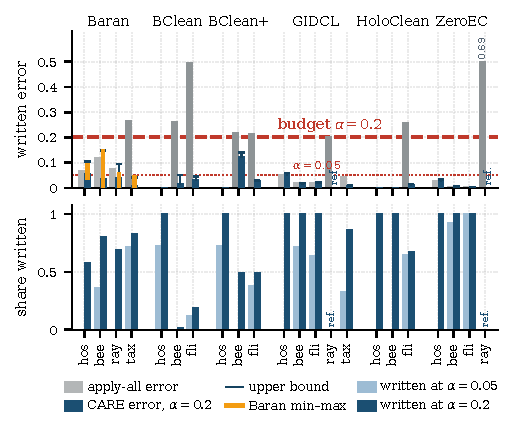
\includegraphics[width=\linewidth]{figures/fig_budget}
  \caption{Per scored pair, the error of writing everything and of what \textsc{Care}
  writes at $\alpha=0.2$ (top) and the share written at $\alpha=0.05$ and $0.2$
  (bottom). Whiskers are Baran's range over six draws.}
  \Description{Two bar-chart panels sharing an x-axis of cleaner--table pairs: on top, apply-all error next to CARE's written error against the budget lines; below, the share of repairs CARE writes at two budgets.}
  \label{fig:pareto}
\end{figure}

\subsection{The bound under corruption and drift}
\label{sec:robust}
Do Propositions~\ref{thm:1} and~\ref{thm:2} describe what happens on real tables? We
inject wrong repairs at controlled rates into five cleaner--table configurations, first
through an untrusted source and then through a trusted one, and finally let the data
drift.

\textbf{Untrusted source (Proposition~\ref{thm:1}).} As the poisoned fraction rises to
$0.2$, none of the poison is written and the error of what \textsc{Care} writes stays
at its clean level. Writing everything, in contrast, degrades by $17$ to $19$ points.

\textbf{Trusted source (Proposition~\ref{thm:2}).} Here no filter can help, so the
question is whether the clean part stays within budget, and it does. Its error was at
most $0.06$ against $\alpha=0.2$ at every contamination level, and the total error
stayed below the bound of Proposition~\ref{thm:2} ($0.191$--$0.233$ against
$0.348$--$0.356$ at the highest level). When we also made up to $0.4$ of the trust
labels wrong, the error never exceeded that bound in $2{,}000$ runs.

\textbf{Drift.} Calibrated on one corruption level of Ni et al.'s beers variants and
deployed on another, Baran's written error reached $0.452$, so assumption (A1) matters
in practice. Re-validating each stratum before committing
(Section~\ref{sec:operate}) brought the budget violations to $0$ of $50$ splits in all
$16$ settings. Where nothing drifted it kept $0.217$ of the $0.221$ written at
$\alpha=0.2$, and $0.075$ of $0.181$ at $\alpha=0.1$, where $30$ audited repairs
tolerate no error.

\section{Why Accuracy and Confidence Are Not Enough}
\label{sec:findings}

This section reports two findings that only become visible once every written
cell is scored and bounded. Cleaners rewrite correct cells
(Sections~\ref{sec:harm} and~\ref{sec:nonoracle}), and no confidence signal can stand in
for the checked sample (Section~\ref{sec:conf}).

\subsection{The cost that repair accuracy does not measure}
\label{sec:harm}

The repair $F_1$-score counts only the cells the benchmark marks as wrong. A cleaner
that chooses which cells to rewrite also changes correct ones, which
Table~\ref{tab:audit} counts in its ``overwr.'' column.

GIDCL on \textsc{rayyan} is the clearest case, because the cleaner is good and the harm
is still visible. On the $948$ error cells it repairs $882$ and is $0.946$ accurate. It
also writes to $176$ cells that were already correct. $151$ of them are in one date
column, where a correct \texttt{1/1/71} becomes \texttt{1/71/01}, a date no parser
reads, and the other $25$ are format-only changes. No declared constraint catches
either kind. Counted over everything GIDCL writes, $226$ of $1{,}108$ values differ from
the clean table, an error of $0.203$, above every budget, so \textsc{Care} admits
nothing (forgiving the $25$ format-only cells leaves $0.181$). The table is still
cleaner after GIDCL, yet one in five of its writes departs from the truth, which is the
figure an unattended operator needs and no repair metric reports.

The pattern is not specific to LLMs or to \textsc{rayyan}. BClean and BClean+ move
flight times by minutes on $156$ and $81$ correct cells (Table~\ref{tab:audit}).

\subsection{With a real detector the budget holds and automation moves}
\label{sec:nonoracle}

\begin{table}[t]
  \centering
  \caption{Oracle versus real detection at $\alpha=0.2$, as the share of repairs
  written and their error, with the real detector's precision and recall. The real
  detector is Raha, or GIDCL's own ($\S$). Bold marks the pairs whose share did not
  fall, and $\ddagger$ logs that also list the cells a cleaner left unchanged. Baran is
  one draw.}
  \label{tab:nonoracle}
  \small
\setlength{\tabcolsep}{4pt}
\renewcommand{\arraystretch}{0.9}
\begin{tabular}{@{}lrrrrrr@{}}
\toprule
& \multicolumn{2}{c}{detector} & \multicolumn{2}{c}{oracle} & \multicolumn{2}{c}{real detector} \\
\cmidrule(lr){2-3}\cmidrule(lr){4-5}\cmidrule(lr){6-7}
Dataset & prec. & rec. & share & error & share & error \\
\midrule
\multicolumn{7}{@{}l}{\emph{Baran}} \\
\quad\textsc{hospital} & 0.92 & 0.45 & $0.86$ & $0.060$ & \emph{refused} & -- \\
\quad\textsc{beers} & 0.74 & 0.84 & $0.80$ & $0.025$ & $\mathbf{0.94}$ & $0.025$ \\
\quad\textsc{flights} & 0.93 & 0.76 & $1.00$ & $0.000$ & $0.68$ & $0.023$ \\
\quad\textsc{rayyan} & 0.84 & 0.80 & $0.77$ & $0.054$ & \emph{refused} & -- \\
\quad\textsc{tax} & 0.81 & 0.77 & $0.73$ & $0.000$ & $\mathbf{0.94}$ & $0.000$ \\
\addlinespace[2pt]
\multicolumn{7}{@{}l}{\emph{BClean}$^{\ddagger}$} \\
\quad\textsc{hospital} & 0.92 & 0.45 & $0.87$ & $0.000$ & $0.62$ & $0.000$ \\
\quad\textsc{beers} & 0.74 & 0.84 & $0.01$ & $0.017$ & $\mathbf{0.08}$ & $0.012$ \\
\quad\textsc{flights} & 0.93 & 0.76 & $0.12$ & $0.034$ & $\mathbf{0.14}$ & $0.029$ \\
\addlinespace[2pt]
\multicolumn{7}{@{}l}{\emph{HoloClean}$^{\ddagger}$} \\
\quad\textsc{hospital} & 0.92 & 0.45 & $0.53$ & $0.000$ & $0.34$ & $0.000$ \\
\quad\textsc{beers} & 0.74 & 0.84 & $0.50$ & $0.000$ & $0.13$ & $0.000$ \\
\quad\textsc{flights} & 0.93 & 0.76 & $0.32$ & $0.014$ & $\mathbf{0.39}$ & $0.014$ \\
\addlinespace[2pt]
\multicolumn{7}{@{}l}{\emph{GIDCL}$^{\S}$} \\
\quad\textsc{hospital} & 1.00 & 1.00 & $1.00$ & $0.054$ & $\mathbf{1.00}$ & $0.054$ \\
\quad\textsc{beers} & 1.00 & 1.00 & $1.00$ & $0.016$ & $\mathbf{1.00}$ & $0.018$ \\
\quad\textsc{flights} & 0.99 & 0.98 & $1.00$ & $0.013$ & $\mathbf{1.00}$ & $0.019$ \\
\quad\textsc{rayyan} & 0.84 & 0.98 & $0.80$ & $0.003$ & \emph{refused} & -- \\
\quad\textsc{tax} & 0.99 & 0.02 & $0.87$ & $0.000$ & $\mathbf{0.87}$ & $0.008$ \\
\addlinespace[2pt]
\bottomrule
\end{tabular}

\end{table}

So far most cleaners were told which cells are wrong. Table~\ref{tab:nonoracle}
replaces that oracle with a real detector, Raha (precision $0.74$--$0.93$, recall
$0.45$--$0.84$) or GIDCL's own. The budget held on all $16$ pairs. Automation moved in
both directions. It was unchanged or higher on $9$ pairs, lower on $4$ and refused on
$3$. Two mechanisms explain the movement.

The first is recall. A detector that misses errors hands the cleaner a different
subset of them. Raha recovers $45\%$ of \textsc{hospital}'s errors and $84\%$ of
\textsc{beers}', and Baran's accuracy moves from $0.932$ to $0.772$ on the first, where
nothing is admissible any more, and from $0.881$ to $0.947$ on the second, where
automation rises.

The second is precision. A detector that flags correct cells hands them to the cleaner,
and cleaners differ in what they do next. Baran changes $62\%$ of the false positives it
is handed on \textsc{flights} and $100\%$ on \textsc{rayyan}, while BClean changes $0\%$
on \textsc{hospital} and \textsc{beers} and $10\%$ on \textsc{flights}. Each change
turns a correct cell into an error. We attribute this to the interface rather than to
the model. A cleaner handed a cell with no way to answer ``nothing to fix'' invents a
change, so the interface must carry an abstention, as the empty \texttt{value} in our
log contract does.

Whatever the detector, the repairs \textsc{Care} wrote never left a table with more
errors than before, and the bound of Corollary~\ref{cor:net} held in all $1{,}080$
seed-runs.

\subsection{Confidence cannot replace the checked sample}
\label{sec:conf}
Why check a sample at all? A simpler rule would write every repair whose score is
above $1-\alpha$. For that rule to work the score must be a calibrated probability, and
it must rank correct repairs first. We tested both on all $\nruns$ cleaner runs in the
study.

\textbf{Confidence is not a probability.} The gap between a cleaner's mean confidence
and the share of its repairs that are actually correct spans $+0.421$ to $-0.887$, and
every cleaner is off by more than $0.1$ on at least one table. Agreement across runs is
no better. ZeroEC's three runs agree on $72\%$ of repairs on \textsc{rayyan}, where it
is $30\%$ right, because the runs agree on the same wrong answer. The decisive case is
HoloClean, the only cleaner that emits a true posterior. All $232$ of its repairs on
hospital are correct, yet it reports posteriors of $0.16$--$0.75$. Thresholding at
$1-\alpha=0.9$ would therefore write \emph{none} of them, whereas \textsc{Care} admits
all of them at $\alpha=0.2$.

\begin{figure}[t]
  \centering
  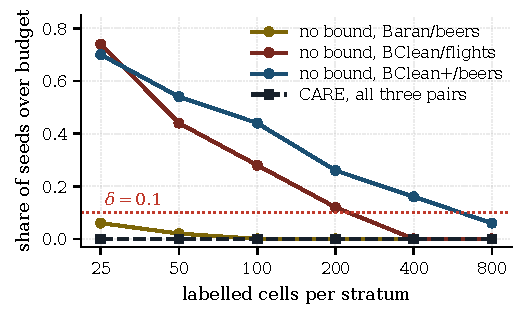
\includegraphics[width=\linewidth]{figures/fig_naive_threshold}
  \caption{Share of seeds in which the budget is broken, against the number of labelled
  cells, when a stratum is accepted on its observed error without a bound and under
  \textsc{Care} ($\alpha=0.1$, $50$ seeds per point). The dotted line is the allowed
  failure rate $\delta$.}
  \Description{Line chart of the fraction of seeds that violate the error budget against the number of labelled calibration cells, for acceptance on observed error without a bound and for CARE, which stays at zero.}
  \label{fig:heldout}
\end{figure}

\textbf{The labels cannot be skipped.} Consider \textsc{Care} without the bound, where
a stratum is accepted whenever its \emph{observed} error is at most $\alpha$. This
naive rule broke the budget in $191$ of $900$ runs, in $74\%$ of the seeds at its worst
point, whereas \textsc{Care} did so in $0$ of $900$ (Fig.~\ref{fig:heldout}).
Recalibrating the scores did not rescue the simple rule either. Isotonic
regression~\cite{zadrozny2002transforming} broke the budget in $40$ of $80$ runs, and
Platt scaling~\cite{Platt1999ProbabilisticOF} kept it only by selecting nothing on
three of four pairs.

\textbf{Confidence does not always order.} \textsc{Care} can admit \emph{part} of a
stratum only when the confidence ranks repairs by correctness. BClean's score does. On
flights its top decile is $0.81$ accurate against $0.47$ for the pool, which is what
lets \textsc{Care} write half of BClean+'s repairs there. GIDCL's score does not, with
an area under the ROC curve of $0.34$--$0.59$. When a score carries no order,
\textsc{Care} accepts or refuses each stratum whole, and a score that cannot order
repairs cannot mislead the decision either.

\section{Limitations and Future Work}
\label{sec:limits}

\textbf{Where \textsc{Care} mostly escalates.} Two regimes leave most of the work to
the reviewer. The first is a wide table with many small columns at a strict budget, where
few strata reach the label floor even after grouping (Table~\ref{tab:labels}). The
second is a table whose distribution shifts faster than batches accumulate, where the
per-stratum audit is paid on every batch. In both regimes
\textsc{Care} escalates and writes nothing beyond its bound. Weighted~\cite{10.48550/arxiv.1904.06019} and
adaptive~\cite{10.48550/arxiv.2106.00170} conformal variants could lower the audit
cost, and we have not evaluated a long sequence of drifting batches.

\textbf{What the bound covers.} The bound is per stratum, marginal over cells and about
exact match, so it ignores a row's joint correctness and counts the $25$ format-only
rewrites as errors. It is also relative to the benchmark's clean tables, whose own
errors (documented for flights and rayyan) affect every cleaner.

\textbf{The study.} Human review is modelled by oracle
labels~\cite{10.14778/1952376.1952378, 10.14778/2994509.2994514}, counted in cells
rather than in time. Only two detectors are sampled, and the one large table, tax, is
synthetic. The two LLM cleaners ran as we could run them, GIDCL from its released
tables with a detector that we retrained, and ZeroEC on a smaller model than its
paper's, which cost it \textsc{rayyan}. None of the six cleaners draws its values
from external sources, so the corruption of Section~\ref{sec:robust} is injected, and
the gate remains to be exercised on a retrieval-based
cleaner~\cite{10.14778/3685800.3685890}. Baran's unseeded active learning makes every
rerun a different cleaner, and the bound held in all $150$ rerun configurations.

\section{Conclusion}

We asked how many of a cleaner's repairs can skip human review at a chosen error rate,
and we answered with error-bounded automation, a number that can be computed for any
cleaner. The usual risk-control methods assume a monotone risk that a cleaner's
confidence does not provide, so the bound rests on an exact test over a fixed grid and
on a design that keeps it valid for an unmodified cleaner under overwrites, corrupted
sources and drift. The budget held in every configuration, whereas unreviewed writing broke it in
$12$ of $21$ pairs at $5\%$, and the bound survived detectable corruption. We draw three
lessons. Suitability for unattended use belongs to the cleaner--table pair, not to the
cleaner alone. What disqualifies a cleaner can be invisible to its accuracy, so
deployment evaluation must score every cell that is written. Confidence is not a
probability and need not order repairs correctly, so governance must be calibrated per
table, and when it is, it fails by refusal rather than by silent corruption.

%\clearpage

%% Acknowledgements (two funding statements, about 10--15 lines) go here:
%\begin{acks}
%\end{acks}

\bibliographystyle{ACM-Reference-Format}
\bibliography{references}

\end{document}
\endinput
